% ============================================================================
%  sections/A2_details.tex --- Appendix B: implementation and experimental
%  details.  This file is an EVIDENCE RECORD, not a second paper: it is
%  organised so that a claim can be looked up, not so that it reads as an
%  argument.  Keep it that way.
%
%  Organisation.  One subsection per object, in the order a reader reproducing
%  the work would need them:
%    B.1  the objectives as implemented (clipping, Huberisation, gradient)
%    B.2  hyperparameters and numerical constants
%    B.3  training scale and hardware
%    B.4  data, preprocessing, perturbation shards, and the shard audit
%    B.5  evaluation protocol
%    B.6  estimator resolution   <-- the highest-risk item; keep it prominent
%    B.7  calibration diagnostics, per-seed tables, teacher-evaluator agreement reference
%    B.8  perturbation families
%    B.9  the matched six-cell grid
%    B.10 the earlier, confounded round, and the two recovered evaluations
%    B.11 the 240-parent replication and its contamination
%    B.12 complete record of evaluations run
%    B.13 de novo generation quality
%    B.14 the capability matrix
%    B.15 numerical stability of the value objective
%    B.16 inferential statistics, collected for completeness (the ONLY place in
%         the manuscript where a t or a p appears; see the reporting policy in
%         B.5 -- descriptive statistics everywhere else, in both directions)
%    B.17 limitations, in full
%    B.18 main-text figures: panel construction
%    B.19 reproduction
%
%  REPEATED CAVEATS ARE CONSOLIDATED (2026-08-29 compression pass).  Each of
%  the following is stated once in the main text and once here, at the anchor
%  named, and is cross-referenced rather than restated anywhere else:
%    q_theta is not the joint conditional      -> ass:A2, limitation (vi-d)
%    the log-variance divergence is prior work -> rem:logvar, App. C
%    the gradient is a truncated-adjoint one   -> app:asimplemented,
%                                                 rem:idealresidual
%    value-arm means are completion-conditional-> app:p0cells reporting rules
%    the objective is local, not basin-mass    -> cor:basins, limitation (iii)
%    kT = 1 eV is numerical, not physical      -> app:hyper, limitation (iv)
%    the likelihood is resolution-dependent    -> app:estimator, limitation (vi)
%  Do not re-add a paragraph restating one of these in a third place.
%
%  PROVENANCE OF NUMBERS.  Every value here is either in the verified list that
%  governs this manuscript, or was recomputed for this pass from the named
%  machine-readable artefact and is labelled as such in the surrounding text.
%  No number in this file is taken from an earlier PDF or from prose.
%
%  ANONYMITY.  No cluster names, no absolute paths, no repository URLs.  Scripts
%  are named by basename only; they are named in the archive described in B.19, which is to be released with the paper.
% ============================================================================

\section{Implementation and Experimental Details}
\label{app:details}

This appendix is the reproducibility record. It states the objectives exactly as
implemented rather than as displayed (\Cref{app:asimplemented,app:hyper}), the
training and evaluation protocols (\Cref{app:hardware,app:data,app:eval}), the
properties of the density estimator that bound how every number may be read
(\Cref{app:estimator}), the full per-seed tables behind each reported mean
(\Cref{app:scalediag,app:p0cells}), the two experimental rounds and the defects of
the earlier one (\Cref{app:p0cells,app:cells}), the auxiliary measurements
(\Cref{app:perturb,app:generation,app:capability}), the numerical-stability record
(\Cref{app:stability}), the complete limitations inventory
(\Cref{app:limitations}), and the reproduction path (\Cref{app:repro}).

\subsection{The objectives as implemented}
\label{app:asimplemented}

The implemented objectives deviate from the displayed ones in ways that are
material, and are listed here rather than left to a reader of the code.

\paragraph{Clipping and Huberisation.} The score read-out of \eqref{eq:score} is
norm-capped at $1000$ per atom before the residual against the teacher force is
formed, and the per-atom squared error is Huberised above $10^{4}$; the anchor term
clamps $\log q_\theta$ at $\pm 10^{6}$; and a value of $\Ls_{\mathrm{value}}$ above
the value-loss cap is rejected outright for that step rather than clipped, because
such values are finite and therefore invisible to a non-finiteness test. The
implemented $\Ls_{\mathrm{force}}$ and $\Ls_{\mathrm{value}}$ are accordingly
clipped and Huberised variants of the stated objectives. All thresholds are in
\Cref{tab:constants}; for a converged model they are inactive.

\paragraph{Frozen-trajectory gradient.} The reverse-time trajectory used for the
continuous-flow log-density is advanced without gradient tracking, each state is
detached before its divergence is taken, and the prior term is computed from a
detached endpoint. The gradient actually back-propagated through
$\Ls_{\mathrm{value}}$ is therefore
\begin{equation}
  \nabla_\theta \Ls_{\mathrm{value}}
  \;\approx\; \sum_{\text{steps}} \Delta t \; \nabla_\theta
  \big(\nabla\!\cdot v_\theta(\vx_{\text{step}}, t_{\text{step}})\big)
  \qquad \text{(trajectory held fixed)} ,
\end{equation}
a truncated-adjoint surrogate: the reverse trajectory and the prior endpoint are held
fixed and only the divergence evaluations are differentiated. We do not differentiate
through the ODE solve, and what the optimiser performs is therefore not exact
likelihood-gradient descent --- neither on the continuous-time likelihood nor on its
discretisation --- but descent on this surrogate.

Three scopes are kept apart throughout the paper, and this paragraph is the place they
meet. \emph{Theory}: the identifiability results of \Cref{app:proofs} characterise the
zero set of the displayed ideal residual objective --- what a model that had driven the
population objective to zero would have been shown, and what that leaves free --- and
make no claim about whether the implemented update converges to that zero set
(\Cref{rem:idealresidual}). \emph{Implementation}: what runs is the finite-step density
estimate of \Cref{app:estimator} optimised by the truncated-adjoint gradient displayed
above, together with the clipping, Huberisation and step rejection listed in this
subsection. \emph{Experiment}: every empirical result in this paper is a measurement of
the behaviour of that implemented procedure, and none of it is offered as evidence about
convergence to the ideal zero set. Where a statement belongs to one scope rather than
another we say so at the statement.

\paragraph{Which code path is live, and what the reported model is.} The reported
value term is the \emph{within-parent} variance of the Boltzmann residual. A
cross-batch variance form also exists in the codebase; it is retained only as a
deprecated reference for unit tests and is mathematically inappropriate here
(\Cref{rem:crossbatch}). In every result reported as ours, the model is the
two-term configuration $\lambda_1 = 0$, $\lambda_3 = 0$,
$\lambda_E = 3\times10^{-5}$: flow matching plus the value term. The gradient term
is defined in \Cref{sec:forcebaseline} because \Cref{sec:ablation} measures it, not
because any reported model uses it; wherever a result comes from a configuration
with $\lambda_1 > 0$ we say so at that result.

\paragraph{The inactive anchor code path.} A third term, $\Ls_{\mathrm{anchor}}$,
exists in the implementation and was inactive ($\lambda_3 = 0$) in \emph{every} run
reported here. It appears in no equation of \Cref{sec:method} and has no experimental
result in this paper; the record is kept because the code path ships, and because it
should not be mistaken for an untried repair of \Cref{sec:scale}. It would constrain
the additive group offset that \eqref{eq:lvalue} cannot see (\Cref{cor:gauge}), and
$\mathrm{NRV}$ is invariant to exactly that offset, so no setting of $\lambda_3$ could
move the calibration endpoint. Its implemented form,
$\mathrm{mean}\,[(\log q_\theta + E/kT + \log \hat Z)^2]$, decomposes into the same
within-group variance the value term already targets plus a squared offset penalty and
introduces no read-out sensitive to the \emph{magnitude} of the density response; and
its predictor $\log \hat Z$ reads element counts, atom count and total charge only, so
it can fix at most one constant per composition rather than the one per group
\Cref{cor:gauge} identifies.

\paragraph{The value estimator as implemented.} \Cref{eq:lvalue} displays
$M^{-1}\sum_m \Var_k(w_{m,k})$. The implementation uses the biased
(divide-by-$K$) variance, drops non-finite residuals, excludes any group left with
fewer than two valid members, and averages over the surviving groups rather than
over $M$; separately, a whole step's value loss is rejected when it exceeds the cap
above, so the optimised objective is a conditionally sampled version of the
displayed one. The null-space statements of \Cref{thm:certificate,cor:gauge} are
unaffected by the biased normalisation --- a variance is annihilated by the same
functions either way --- but they are stated for the full-group objective.

\subsection{Hyperparameters and numerical constants}
\label{app:hyper}
\label{app:constants}

% figures/tabA2_constants.tex --- Table A2 (SPINE Sec. 11 register), appendix.
% Numerical constants that are part of the definition of the losses (SPINE C30).
% Values read from configs/sweep/a*.yaml, cfm_mol/bgfm_loss.py,
% cfm_mol/bgfm_density.py and scripts/fasrc/*.slurm. See the EDITOR-QUERY block
% at the top of sections/A2_details.tex for the items not listed in SPINE Sec.7.7.
% Column widths are tuned to the 5.5in ICLR measure; do not widen.
\begin{table}[t]
\caption{Constants that are part of the definition of the implemented objectives
and of the evaluation protocol. The clipping thresholds are inactive for a
converged model but are part of the objective as trained, so they are stated here
rather than left to the code. Where two settings are listed, ``earlier round'' names the
checkpoint family of \Cref{app:cells} and ``matched grid'' the family of
\Cref{app:p0cells}; the names are family labels and carry no claim that either
configuration achieved numerical stability, which \Cref{app:stability} reports it did
not.}
\label{tab:constants}
\begin{center}
\footnotesize
\setlength{\tabcolsep}{4pt}
\begin{tabular}{@{}p{1.15in}p{1.35in}p{0.95in}p{1.60in}@{}}
\toprule
Symbol / name & Value & Where it acts & Role \\
\midrule
\multicolumn{4}{@{}l}{\emph{Objective}}\\
$\lambda_1$          & $0.1$ (gradient cells), $0$ otherwise & $\Ls_{\mathrm{force}}$ & weight of the gradient-matching term \\
$\lambda_E$ \newline (code field: \texttt{lambda\_2}) & $3\times10^{-5}$ (value cells), $0$ otherwise & $\Ls_{\mathrm{value}}$ & weight of the within-parent Boltzmann-residual variance \\
$\lambda_3$          & $0$ in every reported run & $\Ls_{\mathrm{anchor}}$ & gauge-fixing anchor, inactive \\
$kT$                 & $1.0$ eV ($\approx 11\,600$ K) & both physics terms & temperature scale, not physical \\
$\sigma$             & $1.0$ & prior, read-out & prior standard deviation \\
probe times $t$      & $0.85$, $0.92$, $0.97$ & $\Ls_{\mathrm{force}}$ & amplification $5.7/11.5/32.3\times$ \\
warm-up / ramp       & $1\%$ / $5\%$ of training & schedule & FM only, then a linear ramp \\
\midrule
\multicolumn{4}{@{}l}{\emph{Clipping: the objectives as implemented}}\\
score norm cap       & $1000$ per atom & $s_\theta$ & caps the read-out \\
per-atom error cap   & $10^{4}$ & $\Ls_{\mathrm{force}}$ & Huber transition \\
$\log q_\theta$ clamp & $10^{6}$ & $\Ls_{\mathrm{anchor}}$ & inactive ($\lambda_3 = 0$) \\
value loss cap       & $3000$ (earlier round), $1500$ (matched grid) & $\Ls_{\mathrm{value}}$ & rejects finite outliers \\
\midrule
\multicolumn{4}{@{}l}{\emph{Density estimator}}\\
ODE steps            & 4 train / 12 eval & FFJORD & explicit Euler in state, midpoint-rule divergence quadrature \\
Hutchinson probes    & 2 train / 2 eval & divergence & Rademacher \\
parents per step $M$ & $4$ (earlier round), $8$ (matched grid); $1$ diagnosed only & $\Ls_{\mathrm{value}}$ & estimator variance $\propto 1/M$ \\
step interval        & every 4th step & $\Ls_{\mathrm{value}}$ & amortises the FFJORD cost \\
atoms per parent     & $\leq 50$ & $\Ls_{\mathrm{value}}$ & memory bound \\
\midrule
\multicolumn{4}{@{}l}{\emph{Data and evaluation}}\\
max atoms            & $200$ & preprocessing & molecule size cut \\
elements             & $83$ & preprocessing & bond-free, no bond labels \\
group size $K$       & $5$ train (ref.\ $+\,4$) / $9$ eval (ref.\ $+\,8$) & shards, eval & within-parent groups \\
shard $\sigma$       & $0.03$--$0.40$ \AA{} (5 values) & shards & displacement scales \\
eval $\sigma$        & $0.15$ \AA & eval & perturbation scale \\
parents per arm      & $120$ ($30$ early round) & eval & evaluation groups \\
\bottomrule
\end{tabular}
\end{center}
\end{table}


The physics weights are $\lambda_E = 3\times 10^{-5}$ in the value cells and
$\lambda_1 = 0.1$ in the gradient-supervision cells; $\lambda_3 = 0$ everywhere.
$\lambda_E$ was fixed once from a smoke run, before any density--energy evaluation,
and never tuned against the reported metric: on that run
$\Ls_{\mathrm{value}} \approx 6060$ against $\Ls_{\mathrm{FM}} \approx 0.25$, so the
weight makes $\lambda_E\Ls_{\mathrm{value}} \approx 0.18$, the same order as the
flow-matching term, whereas a ten-fold larger weight would have contributed
$\approx 3.0$ and swamped it. The weight is small; the term's \emph{contribution}
is not, and we use ``lightly weighted'' for the former only.

The temperature scale is $kT = 1.0$~eV ($\approx 11\,600$~K) in every reported
run: it is a numerical choice that keeps $E/kT$ and $F/kT$ tame, not a physical
temperature. Because the variance-form objective is scale-covariant rather than
scale-invariant, the choice of $kT$ fixes the \emph{target within-group slope} of
log-density against energy that the objective asks the model to match; it does not
imply that the trained model represents the Boltzmann distribution over configuration
space as a whole. The score is probed at $t \in \{0.85, 0.92, 0.97\}$ during training; the
prior standard deviation is $\sigma = 1.0$. Physics terms are switched on after a
short flow-matching-only warm-up (1\% of training) and ramped linearly to full
weight over the following 5\%. The value term is evaluated every fourth optimiser
step on parents of at most 50 atoms, which is what makes an FFJORD-based objective
affordable at all.

\subsection{Training scale and hardware}
\label{app:hardware}

Every reported run trains a single bond-free SE(3)-equivariant vector field
(256 hidden scalar channels, 32 vector channels, 6 molecule-update blocks, 32-dim
radial basis to 10~\AA, self-conditioning enabled) on one 141~GB data-centre GPU
with 256~GB of host memory and 16 data-loading workers, using AdamW at base
learning rate $2\times 10^{-4}$, weight decay $10^{-12}$, a 2\% linear warm-up,
gradient-norm clipping at $1.0$, mixed \texttt{bf16} precision, batch size 8 with
two gradient-accumulation steps, for $30\,000$ optimiser steps. Jobs run on a
preemptible partition with a three-day wall clock and resume from the latest
checkpoint on signal. Across the matched grid the cells differ only in the physics
block of the configuration and in the random seed, which is what makes
\Cref{app:p0cells} architecture-matched. The earlier checkpoint family is matched in
architecture, data pipeline, optimiser, schedule and step budget, but not in
parents per value step, loss cap or shard list (\Cref{app:cells}).

\subsection{Data, preprocessing, and the perturbation shards}
\label{app:data}

Training data is the OMol25 4M split \citep{omol25}: 3.9M molecules,
205M atoms, 83 elements, with DFT forces and energies and \emph{no} bond labels.
Preprocessing converts the raw records into flow-matching graphs with
positions, atom-type indices stored as \texttt{int8}, per-atom formal charges, and
per-atom force and per-molecule energy labels read through the standard
single-point-calculator interface. Molecules with more than 200 atoms are
excluded. Bond tensors are written empty and the bond loss weight is zero, so no
bond supervision enters training at any point; where bonds are needed for
evaluation only, they are recovered post hoc from the generated geometry with
\texttt{xyz2mol} \citep{xyz2mol}.

The value term consumes pre-computed perturbation shards rather than the main
data loader. Each shard stores, for each parent molecule, $K = 5$ geometries ---
the data geometry plus four displacements at standard deviations
$\{0.03, 0.06, 0.10, 0.20, 0.40\}$~\AA{} --- together with their teacher energies,
in $K$-contiguous blocks with a parent identifier, so that a within-parent
variance can be formed by reading $K$ consecutive entries. Note that a group
contains the data geometry \emph{together with} its $K-1$ displacements; the
primary endpoint drops the data geometry at evaluation only, never in training.

\paragraph{Composition multiplicity, and why \Cref{cor:basins} does not rest on it.}
Reading the composition of each parent as (element multiset, total charge) from the
stored per-atom types and charges, the $30\,000$-parent training shard carries only
$22\,822$ distinct compositions: $2\,204$ compositions are shared by more than one
parent, covering $9\,382$ parents ($31\%$), at multiplicity up to $80$. It would
therefore be false to describe the supervision design as contributing one group per
composition. What is true, and what \Cref{cor:basins} uses, is that each parent
supplies one empirical perturbation cloud and that clouds sharing a composition
almost surely share no sampled geometry, so the empirical overlap graph is edgeless
whatever the multiplicity. In the evaluated population --- the 120 grid parents and
the 93 primary parents --- every parent does carry a distinct composition, but no
step of the argument uses that.

\paragraph{The shard audit.} Two defects in the shard configuration of the earlier
round are the reason the primary endpoint is defined the way it is, and the reason the
matched grid of \Cref{app:p0cells} was built. Both are stated once, here.

\emph{(a) One shard came from the split the evaluation parents are drawn from.} Every
value arm of the earlier round reads two shards: a $30\,000$-parent shard built from
the training split and a $10\,000$-parent shard built from the validation split. The
density evaluation draws its held-out parents from that same validation split, so
roughly a quarter of the evaluation parents were inside the value term's training pool,
with their true teacher energies, while the flow-matching control --- which disables the
physics block and reads no shard --- was unaffected: the overlap is arm-specific and
favours the arm that wins. Matching each evaluation parent's data geometry back to the
validation file by a translation-invariant signature identifies 118 of 120 parents, 25
of them inside the pool; the remaining 93 are the disjoint set on which the primary
endpoint of \Cref{tab:primary} is computed. The correct repair is to rebuild both shards
from the training split and re-run the arms, which is what the matched grid does: every
cell of \Cref{app:p0cells} reads training-split shards only.

\emph{(b) The earlier scrambled control was scrambled in only one of its two shards.}
The $y$-randomisation control \citep{ruecker2007yrandom} is produced from the
training-split shard by permuting the geometry-to-energy assignment \emph{within} each
parent, so that the energy multiset and the within-parent energy standard deviation
($77.6$~kcal/mol) are bit-for-bit unchanged and only the pairing differs. No scrambled
validation shard was ever built, and that arm's configuration lists the unscrambled
validation shard alongside the scrambled one, so about a quarter of its parent pool
carried true pairings: the negative control was partly a positive control. A second,
smaller defect is that its three seeds are not all configuration-matched to the
true-label arm --- two use $M = 4$ and cap $3000$, matching all four true-label seeds,
and the third uses $M = 8$ and cap $1500$ with batch $4$. Cell C of \Cref{app:p0cells}
repairs both. The general lesson is worth one sentence, because the failure is silent
and reproducible: a $y$-randomisation control is only a control if \emph{every} input it
reads is randomised, and a shard list is exactly the kind of configuration surface on
which that invariant fails without any error being raised.

\subsection{Evaluation protocol}
\label{app:eval}

Local density--energy ordering is measured on held-out parent molecules. The
Stage-1 pipeline emits $K = 9$ geometries per parent: its data geometry, plus 8
copies displaced with per-coordinate standard deviation $\sigma = 0.15$~\AA{}
(centre of mass removed). We compute $\log q_\theta$ for each by reverse-time
integration of the learned flow with 12 first-order steps and a Hutchinson trace
estimator with 2 Rademacher probes per step (\Cref{app:density}). The data geometry
is systematically its group's lowest-energy member and therefore high-leverage, so
the primary endpoint discards it and scores the 8 displaced geometries alone.

Because the evaluation pipeline aggregates to per-group correlations and discards
the individual $(\log q_\theta, E)$ pairs, we re-scored every geometry in every
arm and recompute every reported statistic from that per-record source, composing
the group-to-validation-index map of the contamination check with the
reference-exclusion logic. The re-scoring loses 6 of 1080 single points per arm
rather than the pipeline's 1--2, which shifts a mean by at most $0.004$. Since
every reported number comes from the single re-scored source, they are mutually
comparable.

Each geometry is then scored with GFN2-xTB \citep{gfn2xtb}, a semi-empirical method
\emph{independent} of the neural potential used for training: it enters no training
loss and shares no parameters, data or functional form with the teacher. Of the
1080 attempted geometries per arm, 1078--1080 were scored; the one or two single
points that failed to converge were dropped from their group before the correlation
was formed. We report the Pearson correlation between $\log q_\theta$ and
$-E_{\text{GFN2-xTB}}/kT$ computed \emph{within} each parent and then averaged over
parents. Grouping is not a stylistic choice: pooling all parents into one
regression gives $r^2 = 0.11$ for the value arm and $0.01$ for the flow-matching
control, because between-molecule $\log Z$ offsets dominate the pooled variance
(\Cref{rem:crossbatch}).

\paragraph{How comparisons are reported.} The unit of replication is a training run.
We report effect sizes, means and standard errors over independently trained seeds,
together with every seed-level result. Because several cells contain only two to five
completed seeds and completion is objective-dependent (\Cref{app:stability}), we use
these descriptive quantities rather than treating asymptotic null-hypothesis tests as
the primary evidence. Every arm-level number in this paper is therefore an arm mean
$\pm$ the standard error over seeds, quoted with the number of seeds behind it and,
wherever completion differs by arm, with the launched, completed and diverged counts;
every comparison is quoted as the absolute difference $\Delta r$ of two such means and
read against the observed seed ranges, which the per-seed tables print in full. The
inferential statistics computed during the analysis are collected once, for
completeness and in one place, in \Cref{tab:inferential}; no claim in this paper is
stated in terms of them.

Five seed configurations were prepared for the flow-matching and
value arms and seven for the scrambled arm, of which five, four and three are
reported, and the reasons differ by arm rather than sharing one cause.

All five flow-matching seeds completed and all five are scored, the fifth having
carried no score under this protocol until it was scored under it (\Cref{app:cells}).
The unreported value run and two of the unreported scrambled runs diverged to
non-finite weights before the training budget was reached and were not replaced; a
further scrambled run diverged after its mid-budget checkpoint, which is not the
reported budget and is not scored; and one scrambled run completed with finite weights
but lost its evaluation to a launcher path fault and has since been recovered
(\Cref{app:cells}).

\paragraph{Adverse imputation for the unreported run.}
\label{app:imputation}
The adverse imputation charges the value arm alone, the control arm having no
unreported run left to impute. On the primary endpoint the value arm's four completed
seeds score $0.316$, $0.378$, $0.426$ and $0.358$ and the control arm's five score
$0.222$, $0.194$, $0.249$, $0.142$ and $0.192$, giving arm means $0.369$ and $0.200$
and an observed difference of $\Delta r = +0.169$ (\Cref{tab:scaleseeds}). Two
imputations replace the value arm's one diverged run with a value chosen against us
and recompute that arm's mean over five entries rather than four. \emph{(i)} Imputed at
the control arm's own mean, $0.200$, the value arm falls to $0.336$ and the difference
to $\Delta r = +0.135$. \emph{(ii)} Imputed at the worst value observed in \emph{any}
arm of the round, $0.142$ --- the control arm's fourth seed, and by construction the
most adverse single value available, since no arm of the round produced a lower one ---
the value arm falls to $0.324$ and the difference to $\Delta r = +0.124$. Under both
imputations the imputed five-entry value-arm mean still lies above every one of the
five control seeds, whose maximum is $0.249$. The two conservative imputations are
reported here and referenced from \Cref{sec:mainresult}.

\subsection{Estimator resolution: what the step count controls, and what it does not}
\label{app:estimator}

\Cref{app:density} settles the fact this subsection measures. The reverse solve is
explicit Euler in the \emph{state} over the whole of $[0,1]$, with the divergence
integral taken by the midpoint rule on the same interval: all $n$ quadrature nodes are
interior to $[0,1]$, but the interval itself is not truncated. Every step count
therefore targets one and the same quantity, $\log q_\theta$ at $t = 1$, and refining
$n$ estimates that quantity \emph{more accurately} rather than measuring a different
one. What the step count controls is accuracy, not identity. Any step-count dependence
in the numbers below is accordingly a property of the finite-step readout rather than of
the target. It is dominated by numerical discretisation error --- the $O(\Delta t)$ Euler
state integration, the quadrature being $O(\Delta t^{2})$ and exact for integrands linear
in $t$ --- together with whatever endpoint stiffness the learned field carries and any
step-count-dependent contribution from the stochastic trace term. The certificate the objective can enforce is a statement about
$\log q_\theta$ as formed at a finite step count, and so carries that bias
(\Cref{rem:epscert}). Three consequences follow, in increasing order of how
much they cost us.

\begin{table}[h]
\caption{The integration grid at the three step counts used or examined in this paper.
The three rows are three \emph{accuracies of one quantity}, not three quantities: the
largest node sits at $t_0 = 1 - \Delta t/2$, but the interval integrated is the whole of
$[0,1]$ in every row, so all three target $\log q_\theta$ at $t = 1$
(\Cref{app:density}). The half-step offset keeps the field from being evaluated at
$t = 1$ without moving the endpoint the scheme targets.}
\label{tab:stepgrid}
\begin{center}
\footnotesize
\begin{tabular}{cccc l}
\toprule
$n$ & $\Delta t = 1/n$ & largest node $t_0$ & smallest node $t_{n-1}$ & used for \\
\midrule
$4$  & $0.2500$ & $0.8750$ & $0.1250$ & the training value term ($\Ls_{\mathrm{value}}$) \\
$12$ & $0.0833$ & $0.9583$ & $0.0417$ & every reported evaluation in this paper \\
$48$ & $0.0208$ & $0.9896$ & $0.0104$ & the no-plateau measurement below \\
\bottomrule
\end{tabular}
\end{center}
\end{table}

\paragraph{No plateau over the step counts we can afford, and the measurement that
shows it.} A well-defined target is not the same thing as a converged estimate of it.
Re-scoring the same ten held-out molecules at the three step counts of
\Cref{tab:stepgrid} gives mean $\log q_\theta$ of $-65.5$ ($n = 4$), $-114.3$ ($n = 12$)
and $-199.9$ ($n = 48$): each refinement moves the estimate by a further $49$ and then
$86$ nats, with no sign of a plateau. Under the corrected reading of the scheme these
three numbers are three estimates of the \emph{same} quantity, so their spread is error in
the finite-step readout and not a change of target, and it is large and not visibly decaying
at the resolutions we can pay for. That is consistent with an $O(\Delta t)$ Euler bias against
a field that is stiff near $t = 1$ --- the conditional path has variance
$(1-t)^2\sigma^2 \to 0$ there, so the state integration is least accurate exactly where
the trajectory ends --- but we have not measured the error against an exact reference on
these molecules and we quote no convergence rate for them. We report the sweep as a
disclosure and not as a convergence study: ten molecules is a small sample, and the point
it establishes is that no statement of the form ``$\log q_\theta$ is converged at $n$
steps'' is available for this implementation. What the sweep does \emph{not} show is a
change of target: the three columns differ in accuracy, not in what they estimate.

\paragraph{Training and evaluation run at different discretisation accuracies.} The
value term is evaluated at $n = 4$ because an FFJORD objective inside the training loop
is otherwise unaffordable, while every reported evaluation runs at $n = 12$. Both target
the same quantity, $\log q_\theta$ at $t = 1$; what differs is how much Euler bias each
carries, and the training-time estimate carries more. On the analytic linear-flow check
of \Cref{app:density}, where the endpoint log-density is available in closed form, this
integrator's error is $1.5\times10^{-1}$ at $n = 4$ against $4.7\times10^{-2}$ at
$n = 12$; on real molecules, where the field is learned rather than linear, the sweep
above shows the bias is far from exhausted at either count. The objective therefore
constrains a less accurately estimated log-density than the metric measures. This is a
defect of the implementation rather than of the objective, and it is recorded as a
limitation (\Cref{app:limitations} item (vi)) rather than argued away.

\paragraph{The preliminary check, and why it settles nothing.} A first look at the
resolution dependence re-scored two arms --- the value arm and the flow-matching
control --- at more than one step count on ten parents with one seed per arm. It is
reported here in full, with its precision stated, because that precision is inadequate
and because it is where the resolution sensitivity analysed in the rest of this
subsection was first noticed.

\begin{table}[h]
\caption{Preliminary resolution check: mean per-parent correlation $r$, data
geometry dropped, \textbf{10 parent molecules and one seed per arm}. The per-arm
$\mathrm{SEM}(r) \approx 0.065$, so the standard error of a gap is $\approx 0.095$,
of the same order as the $n = 12$ gap itself, and with a single seed per arm there are
no seed ranges to compare.
``Attenuation-corrected'' rescales each gap by the estimator noise measured from repeat
scoring; the trend is unchanged by it and the signal-to-noise column rises with $n$.
This table may not be compared with \Cref{tab:primary}, and it is superseded at every
resolution by \Cref{tab:respaired}, which scores five flow-matching seeds and four
value seeds on 120 parents at $n = 4$, $12$ and $48$.}
\label{tab:resolution}
\begin{center}
\footnotesize
\begin{tabular}{lccccc}
\toprule
$n$ & value arm & FM-only & gap & gap, atten.-corrected & signal-to-noise \\
\midrule
$4$   & $0.628$ & $0.259$ & $+0.369$ & $+0.465$ & $1.447$ \\
$12$  & $0.347$ & $0.163$ & $+0.183$ & $+0.193$ & $2.631$ \\
\bottomrule
\end{tabular}
\end{center}
\end{table}

\paragraph{The expanded ablation: protocol.} The multi-seed version re-scores existing
checkpoints --- four seeds of the value arm and five of the flow-matching arm --- at
$n \in \{4, 12, 48\}$ on 120 parent molecules with 8 displacements each. Every one of
those nine checkpoints is scored at every one of the three step counts, so the design
is complete and strictly paired, and the seed counts are the same in every row. Three
properties make it a paired design rather than a set of independent evaluations.
\emph{(i)} The evaluation seed is pinned to a
single value across step counts, so the parents drawn from the held-out split and
the Gaussian displacements applied to them are \emph{byte-identical} at every
resolution: a difference between rows of \Cref{tab:respaired} cannot be a
difference in the molecules or in the noise realisation. \emph{(ii)} The checkpoints
scored in one row are scored in the other two, so a difference between rows cannot be a
difference in the models either. The step count is the only configured variable, so the
comparison measures the sensitivity of the complete finite-step stochastic readout: that
sensitivity is dominated by state-integration discretisation, but it also includes any
step-count-dependent variation in the stochastic trace term, since the readout draws two
Rademacher probes per step and the repeat-to-repeat probe spread has not been measured on
this population (\Cref{app:density}). \emph{(iii)} The data geometry is dropped and the per-group
correlation formed exactly as in \Cref{app:eval}, so the rows are commensurable with
\Cref{tab:primary,tab:p0seeds}. The launcher refuses to score a checkpoint
containing any non-finite parameter, a check added after an earlier round evaluated
a corrupted checkpoint (\Cref{app:stability}). Nothing about the estimator was
modified to produce any of this: it re-scores checkpoints that already exist.

\begin{table}[h]
\caption{The strictly paired resolution ablation: mean per-group $r$ by
integrator step count, 120 parents, data geometry dropped, evaluation seed pinned so
that every row scores \emph{identical} molecules and displacements with
\emph{identical} checkpoints. Four value seeds and five flow-matching seeds are scored
at each of the three step counts; the counts in the column heads are those arm sizes
and they do not change down the table. Entries are arm means over independently trained
seeds $\pm$ the standard error over those seeds, and $\Delta r$ is the difference of the
two arm means at that resolution. All three rows
estimate the same quantity and differ only in how accurately they estimate it, so a
difference between them is a difference in finite-step estimation
error, not in target (\Cref{app:density}). \Cref{tab:reschk} gives the per-checkpoint
values behind these means, and \Cref{fig:resolution} draws them. This table supersedes
\Cref{tab:resolution}.}
\label{tab:respaired}%
% alias: earlier drafts and the main text may cite this float as tab:respowered.
\label{tab:respowered}
\begin{center}
\footnotesize
\begin{tabular}{lcccc}
\toprule
$n$ & $\Delta t = 1/n$ & value arm (4 seeds) & FM-only (5 seeds) & $\Delta r$ \\
\midrule
$4$ \ (the training resolution) & $0.2500$ & $+0.571 \pm 0.038$ & $+0.189 \pm 0.014$ & $+0.382$ \\
$12$ (every reported number)    & $0.0833$ & $+0.418 \pm 0.033$ & $+0.204 \pm 0.008$ & $+0.215$ \\
$48$                            & $0.0208$ & $+0.306 \pm 0.011$ & $+0.269 \pm 0.016$ & $+0.037$ \\
\bottomrule
\end{tabular}
\end{center}
\end{table}

\begin{table}[h]
\caption{Per-checkpoint values behind \Cref{tab:respaired}: mean per-group $r$ for
each scored checkpoint at each step count, on the same 120 parents with the same pinned
displacements. Seed labels are within-arm and do not pair across arms. The two arms
respond to refinement in opposite directions: all four value checkpoints fall
monotonically as $n$ increases, while three of the five flow-matching checkpoints rise
monotonically and the other two dip at $n = 12$ before rising, so that all five end higher
at $n = 48$ than at $n = 4$.}
\label{tab:reschk}
\begin{center}
\footnotesize
\setlength{\tabcolsep}{6pt}
\begin{tabular}{llccc}
\toprule
Arm & seed & $n = 4$ & $n = 12$ & $n = 48$ \\
\midrule
\textbf{Value}
 & 1 & $0.528$ & $0.328$ & $0.287$ \\
 & 2 & $0.614$ & $0.433$ & $0.289$ \\
 & 3 & $0.654$ & $0.485$ & $0.320$ \\
 & 5 & $0.489$ & $0.428$ & $0.330$ \\
 & \emph{mean} & $0.571$ & $0.418$ & $0.306$ \\
\midrule
Flow matching only
 & 1 & $0.141$ & $0.199$ & $0.239$ \\
 & 2 & $0.226$ & $0.221$ & $0.315$ \\
 & 3 & $0.176$ & $0.191$ & $0.238$ \\
 & 4 & $0.205$ & $0.183$ & $0.298$ \\
 & 5 & $0.197$ & $0.224$ & $0.257$ \\
 & \emph{mean} & $0.189$ & $0.204$ & $0.269$ \\
\bottomrule
\end{tabular}
\end{center}
\end{table}

% The paired resolution trajectories, drawn from the same per-checkpoint values
% tabulated immediately above.  Generator: figures/figA_resolution.py, which
% recomputes every aggregate and refuses to draw unless it reproduces them.
% figures/figA_resolution.tex -- float wrapper for the APPENDIX resolution figure.
%
% NOT YET INPUT ANYWHERE.  This wrapper is written and ready; the section editor
% adds it to the appendix (Appendix B.6, the numerics discussion) with
%     % figures/figA_resolution.tex -- float wrapper for the APPENDIX resolution figure.
%
% NOT YET INPUT ANYWHERE.  This wrapper is written and ready; the section editor
% adds it to the appendix (Appendix B.6, the numerics discussion) with
%     % figures/figA_resolution.tex -- float wrapper for the APPENDIX resolution figure.
%
% NOT YET INPUT ANYWHERE.  This wrapper is written and ready; the section editor
% adds it to the appendix (Appendix B.6, the numerics discussion) with
%     \input{figures/figA_resolution}
% It must NOT go in the main text: the nine-page main text has no vertical slack
% and this figure is a diagnostic, not a result.
%
% Image produced by figures/figA_resolution.py, which also writes
% figures/out/figA_resolution_data.json recording every number drawn.
%
% PROVENANCE.  The per-checkpoint values are the authoritative re-scoring of the
% records under runs/eval_res/{a1_fm_only,a3_energy_only}[_s<N>]__ode{4,12,48};
% they are transcribed, not recomputed, per the standing instruction.  The
% generator recomputes every AGGREGATE (arm means, gaps, Welch t) from those
% per-checkpoint values and refuses to draw unless each reproduces the
% authoritative aggregate; it also checks the two directional counts the figure
% states before stating them.  The Welch t values stay inside that gate and
% inside figA_resolution_data.json: NO t value and NO significance label is
% rendered in the image or in the caption.  Panel (b) is descriptive -- the
% difference of arm means with the propagated SEM over seeds.
%
% Drawn at final size (5.5 x 2.42 in) with an explicit, non-tight bounding box;
% include with width=\linewidth, never \resizebox.
\begin{figure}[t]
\begin{center}
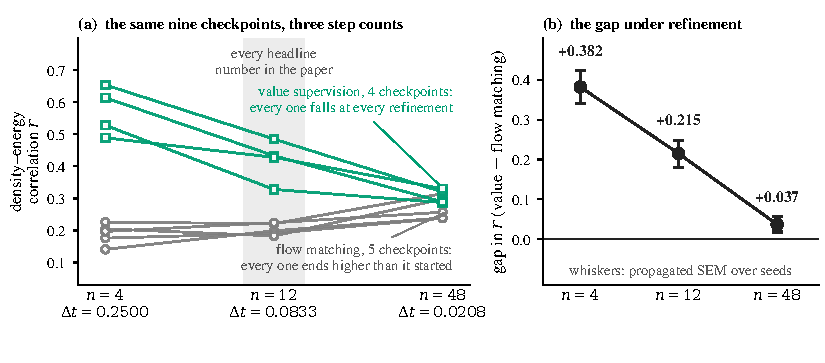
\includegraphics[width=\linewidth]{figures/out/figA_resolution.pdf}
\end{center}
\caption{\textbf{The paired resolution sweep.} The same nine checkpoints ---
five flow-matching controls (seeds $1$--$5$) and four value runs (seeds
$1$, $2$, $3$, $5$) --- re-scored at $n = 4$, $n = 12$ and $n = 48$ ODE steps on
identical parents, identical displacements and a pinned evaluation seed.
\textbf{(a)} Per checkpoint: all four value checkpoints fall at every
refinement, and all five flow-matching checkpoints end higher at $n = 48$ than
at $n = 4$, three of them monotonically. \textbf{(b)} The arm gap decays
$+0.382 \rightarrow +0.215 \rightarrow +0.037$. Each point is the difference of
the two arm means over independently trained seeds, five control and four
value, and each whisker is the propagated standard error over those seeds, a
descriptive SEM rather than a confidence interval. Every number reported
elsewhere in the paper is computed at $n = 12$. The value loss was itself
computed at $n = 4$, so one reading of the decay is that the ordering the term
teaches is expressed most strongly in the object the coarse estimator reports;
that is offered as a reading and not as a demonstrated mechanism. What the
analysis establishes is that the estimator is sensitive to solver resolution.
It does not distinguish model-dependent numerical error from an effect learned
under the four-step training estimator.}
\label{fig:resolution}
\end{figure}

% It must NOT go in the main text: the nine-page main text has no vertical slack
% and this figure is a diagnostic, not a result.
%
% Image produced by figures/figA_resolution.py, which also writes
% figures/out/figA_resolution_data.json recording every number drawn.
%
% PROVENANCE.  The per-checkpoint values are the authoritative re-scoring of the
% records under runs/eval_res/{a1_fm_only,a3_energy_only}[_s<N>]__ode{4,12,48};
% they are transcribed, not recomputed, per the standing instruction.  The
% generator recomputes every AGGREGATE (arm means, gaps, Welch t) from those
% per-checkpoint values and refuses to draw unless each reproduces the
% authoritative aggregate; it also checks the two directional counts the figure
% states before stating them.  The Welch t values stay inside that gate and
% inside figA_resolution_data.json: NO t value and NO significance label is
% rendered in the image or in the caption.  Panel (b) is descriptive -- the
% difference of arm means with the propagated SEM over seeds.
%
% Drawn at final size (5.5 x 2.42 in) with an explicit, non-tight bounding box;
% include with width=\linewidth, never \resizebox.
\begin{figure}[t]
\begin{center}
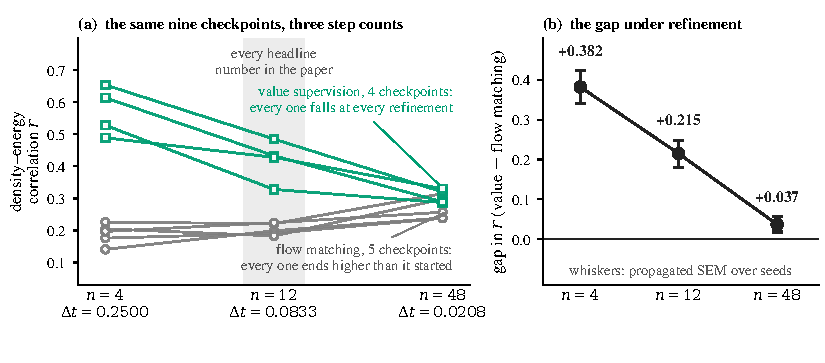
\includegraphics[width=\linewidth]{figures/out/figA_resolution.pdf}
\end{center}
\caption{\textbf{The paired resolution sweep.} The same nine checkpoints ---
five flow-matching controls (seeds $1$--$5$) and four value runs (seeds
$1$, $2$, $3$, $5$) --- re-scored at $n = 4$, $n = 12$ and $n = 48$ ODE steps on
identical parents, identical displacements and a pinned evaluation seed.
\textbf{(a)} Per checkpoint: all four value checkpoints fall at every
refinement, and all five flow-matching checkpoints end higher at $n = 48$ than
at $n = 4$, three of them monotonically. \textbf{(b)} The arm gap decays
$+0.382 \rightarrow +0.215 \rightarrow +0.037$. Each point is the difference of
the two arm means over independently trained seeds, five control and four
value, and each whisker is the propagated standard error over those seeds, a
descriptive SEM rather than a confidence interval. Every number reported
elsewhere in the paper is computed at $n = 12$. The value loss was itself
computed at $n = 4$, so one reading of the decay is that the ordering the term
teaches is expressed most strongly in the object the coarse estimator reports;
that is offered as a reading and not as a demonstrated mechanism. What the
analysis establishes is that the estimator is sensitive to solver resolution.
It does not distinguish model-dependent numerical error from an effect learned
under the four-step training estimator.}
\label{fig:resolution}
\end{figure}

% It must NOT go in the main text: the nine-page main text has no vertical slack
% and this figure is a diagnostic, not a result.
%
% Image produced by figures/figA_resolution.py, which also writes
% figures/out/figA_resolution_data.json recording every number drawn.
%
% PROVENANCE.  The per-checkpoint values are the authoritative re-scoring of the
% records under runs/eval_res/{a1_fm_only,a3_energy_only}[_s<N>]__ode{4,12,48};
% they are transcribed, not recomputed, per the standing instruction.  The
% generator recomputes every AGGREGATE (arm means, gaps, Welch t) from those
% per-checkpoint values and refuses to draw unless each reproduces the
% authoritative aggregate; it also checks the two directional counts the figure
% states before stating them.  The Welch t values stay inside that gate and
% inside figA_resolution_data.json: NO t value and NO significance label is
% rendered in the image or in the caption.  Panel (b) is descriptive -- the
% difference of arm means with the propagated SEM over seeds.
%
% Drawn at final size (5.5 x 2.42 in) with an explicit, non-tight bounding box;
% include with width=\linewidth, never \resizebox.
\begin{figure}[t]
\begin{center}
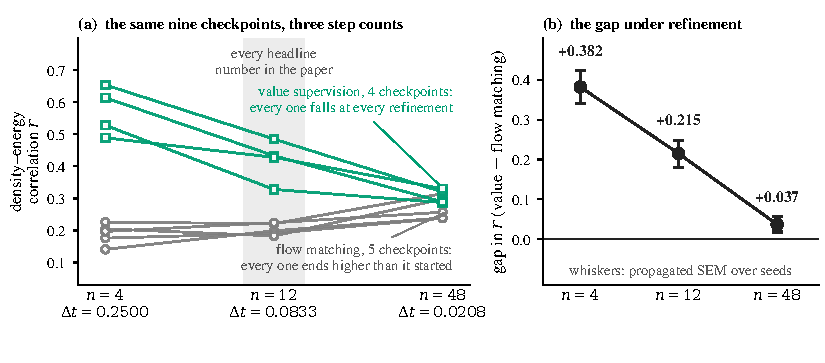
\includegraphics[width=\linewidth]{figures/out/figA_resolution.pdf}
\end{center}
\caption{\textbf{The paired resolution sweep.} The same nine checkpoints ---
five flow-matching controls (seeds $1$--$5$) and four value runs (seeds
$1$, $2$, $3$, $5$) --- re-scored at $n = 4$, $n = 12$ and $n = 48$ ODE steps on
identical parents, identical displacements and a pinned evaluation seed.
\textbf{(a)} Per checkpoint: all four value checkpoints fall at every
refinement, and all five flow-matching checkpoints end higher at $n = 48$ than
at $n = 4$, three of them monotonically. \textbf{(b)} The arm gap decays
$+0.382 \rightarrow +0.215 \rightarrow +0.037$. Each point is the difference of
the two arm means over independently trained seeds, five control and four
value, and each whisker is the propagated standard error over those seeds, a
descriptive SEM rather than a confidence interval. Every number reported
elsewhere in the paper is computed at $n = 12$. The value loss was itself
computed at $n = 4$, so one reading of the decay is that the ordering the term
teaches is expressed most strongly in the object the coarse estimator reports;
that is offered as a reading and not as a demonstrated mechanism. What the
analysis establishes is that the estimator is sensitive to solver resolution.
It does not distinguish model-dependent numerical error from an effect learned
under the four-step training estimator.}
\label{fig:resolution}
\end{figure}


\paragraph{What it settles, and what it does not.} Three observations, stated
descriptively. \emph{(a) The gap is present at the resolution we report.} At $n = 12$
the two arm means are $+0.418 \pm 0.033$ over four value seeds and $+0.204 \pm 0.008$
over five control seeds, for $\Delta r = +0.215$; the four value checkpoints span
$0.328$--$0.485$ and the five control checkpoints span $0.183$--$0.224$, so the two
observed seed ranges do not overlap. The same checkpoints scored under the paper's own
evaluation draw give $+0.182$ on the same 120-parent, geometry-dropped population
(\Cref{tab:scaleperm}, block 2: $0.397$ against $0.215$). The two agree in sign and in
size to within $0.033$, which is a consistency check and not an independent
replication: the checkpoints are one family, and what differs is the pinned evaluation
draw. \emph{(b) The magnitude of the observed gap decreases as the finite-step
estimator is refined.} It is $+0.382$ at $n = 4$, $+0.215$ at $n = 12$ and $+0.037$ at
$n = 48$. At $n = 48$ the two observed seed ranges do overlap: the value checkpoints
span $0.287$--$0.330$ and the control checkpoints $0.238$--$0.315$. Every headline
number in this paper is computed at $n = 12$. \emph{(c) The two arms move in opposite
directions under refinement.} The value arm falls from $+0.571$ to $+0.306$ while the
flow-matching arm rises from $+0.189$ to $+0.269$, and \Cref{tab:reschk} shows the split
holds checkpoint by checkpoint: all four value checkpoints fall at every refinement,
and all five control checkpoints end higher at $n = 48$ than at $n = 4$, three of them
monotonically.

One reading we offer --- as a reading, not as an established mechanism --- is that the
value loss was itself computed at $n = 4$, and so shaped the object the $n = 4$
estimator reports: the model would then have learned to order the density at the
resolution its training objective could see, and that ordering would weaken as the
estimate is refined. What this analysis establishes is estimator-resolution
sensitivity: it does not distinguish model-dependent numerical error from an effect
learned specifically under the four-step training estimator, and the observed
arm-dependent trends are consistent with either. Whichever the source, the effect size
is a property of the pair (model, step count) and not of the model alone, which is why
every number in this paper is quoted with the step count it was computed at, and why
the $n = 48$ row is reported here in full rather than summarised.

\paragraph{The second resolution family, and why it is supporting rather than
primary.} A second complete re-scoring at more than one step count exists in the run
store, on the checkpoints of the matched grid rather than on the earlier arms: cells A
and D of \Cref{app:p0cells} were re-scored at $n = 4$ and $n = 48$ under the same
geometry-dropped, 120-parent convention. It is listed here with its values and its
coverage rather than set aside without one, and \Cref{tab:resother} gives it in full.
Two properties keep it out of the primary comparison and neither is a matter of
preference. First it is \emph{incomplete in the step dimension}: it carries $n = 4$ and
$n = 48$ but no $n = 12$ row, so it cannot be read at the resolution every reported
number in this paper uses, and it supplies two points of a curve rather than three.
Second its value arm is drawn from a \emph{different seed set} from the matched design:
its six D checkpoints are the three matched-block seeds together with three of the
later independently launched seeds, which the reporting rules of \Cref{app:p0cells}
forbid merging into a matched-grid mean. It is also a different evaluation draw from
the family of \Cref{tab:respaired}, being scored on the grid's own parents and
displacements rather than on the earlier round's, so the two families' rows are not
byte-paired with one another even though each is internally paired across step counts.
We therefore classify it as \emph{supporting evidence for the numerical sensitivity of
the estimator}, not as a second matched primary comparison, and no contrast in this
paper is formed from it. What it adds is that the same two directions appear on an
independent set of checkpoints: between $n = 4$ and $n = 48$ the value-carrying cell
falls from $+0.614$ to $+0.314$ while the physics-free cell rises from $+0.161$ to
$+0.261$, and the difference of arm means falls from $+0.453$ to $+0.053$.

\begin{table}[h]
\caption{The second, supporting resolution family: cells A and D of the matched grid
(\Cref{app:p0cells}) re-scored at two step counts, 120 parents, data geometry dropped,
GFN2-xTB, evaluation seed pinned across step counts within this family. Entries are arm
means over checkpoints $\pm$ the standard error over checkpoints, with every
per-checkpoint value printed beside them. This family is \textbf{not} a matched primary
comparison and no contrast in this paper is formed from it: it carries no $n = 12$ row,
so it cannot be read at the resolution the paper reports, and its D arm mixes the three
matched-block seeds ($s2$, $s3$, $s5$) with three later independently launched seeds
($s6$, $s7$, $s9$), which the reporting rules of \Cref{app:p0cells} keep separate. It is
recorded as supporting evidence for the estimator's resolution sensitivity.
Recomputed for this table from the family's own per-record evaluation outputs by the
same per-group routine that produces \Cref{tab:reschk}.}
\label{tab:resother}
\begin{center}
\footnotesize
\setlength{\tabcolsep}{5pt}
\begin{tabular}{llcc}
\toprule
Cell & per-checkpoint $r$ & mean $\pm$ SEM & \\
\midrule
\multicolumn{4}{@{}l}{\emph{$n = 4$ (the training resolution)}} \\
D \texttt{energy} (6 ckpts) & $0.652$, $0.647$, $0.592$, $0.618$, $0.569$, $0.605$ & $+0.614 \pm 0.013$ & \\
A \texttt{fmonly} (5 ckpts) & $0.174$, $0.137$, $0.165$, $0.188$, $0.142$ & $+0.161 \pm 0.010$ & \\
 & & $\Delta r = +0.453$ & \\
\midrule
\multicolumn{4}{@{}l}{\emph{$n = 12$}} \\
\multicolumn{3}{@{}l}{\emph{not scored in this family}} & \\
\midrule
\multicolumn{4}{@{}l}{\emph{$n = 48$}} \\
D \texttt{energy} (6 ckpts) & $0.358$, $0.308$, $0.347$, $0.271$, $0.297$, $0.301$ & $+0.314 \pm 0.013$ & \\
A \texttt{fmonly} (5 ckpts) & $0.229$, $0.269$, $0.273$, $0.290$, $0.243$ & $+0.261 \pm 0.011$ & \\
 & & $\Delta r = +0.053$ & \\
\bottomrule
\end{tabular}
\end{center}
\end{table}

\paragraph{What would actually settle it.} There is no coupling defect to repair here:
the scheme integrates over the whole of $[0,1]$ and targets $\log q_\theta$ at $t = 1$
at every step count. What there is instead is bias --- first order in $\Delta t$ from
the Euler state integration against $O(\Delta t^2)$ from the quadrature --- and no step
count reported in this paper demonstrates a plateau, so we claim convergence for none
of these numbers. The missing measurements are the ordinary numerical ones: a
higher-order or adaptive integrator for the state, and more steps at both training and
evaluation time until the reported value stops moving. To those the opposite-direction
result of \Cref{tab:reschk} adds one more: an arm whose value term is computed at the
resolution the evaluation uses, which is the comparison that would separate the
solver's contribution from what the coarse objective taught. We have not run them, and
no result in this paper reflects them.

\subsection{Calibration diagnostics, per-seed values, and the teacher-evaluator agreement reference}
\label{app:scalediag}

This subsection gives the definitions behind the calibration endpoint, every
per-seed value behind every mean in \Cref{tab:primary} and \Cref{fig:calibration},
the sensitivity of those numbers to the two evaluation corrections, and how the
teacher-evaluator agreement reference is measured.

% ---------------------------------------------------------------------------
%  RELOCATED FROM THE MAIN TEXT BY THE 2026-08-19 COMPRESSION PASS.  This was
%  Table 1 of the pre-compression manuscript; the caption is unchanged apart
%  from cross-references that pointed at main-text floats.  Every number it
%  carries is also stated in the prose of Sec. 5.2 and Sec. 5.3.
% ---------------------------------------------------------------------------
\begin{table}[h]
\caption{\textbf{The primary endpoint}: 93 held-out parents disjoint from the value term's shard
pool, data geometry dropped, $8$ displaced geometries each, every energy a GFN2-xTB single point
from an evaluator independent of the eSEN training teacher. $r$ is the per-parent correlation between $\log q_\theta$, the clamped positional-flow density,
and $-E/kT$, averaged over parents then seeds ($\pm$ SEM over seeds);
$\mathrm{NRV}$ \eqref{eq:rm} is the median over parents per seed, then the mean over seeds, and is
anchored: \textbf{a constant log-density scores exactly $1$}. $kT_{\mathrm{eff}}$ ideally equals
the $1.0$~eV training target, and retrieval is against $12.5\%$ and $37.5\%$ at chance. The last row is
\emph{not a model} but the teacher's own energies through the identical pipeline, reported for $r$
and retrieval only; it is a reference for what exact reproduction of the teacher would score on
this ensemble, not an attainable maximum, and its calibration diagnostics are derived in
\Cref{fig:calibration}. $^{\dagger}$The scrambled row is a defective control, one of its two shards
having been left unscrambled and its third seed not configuration-matched, and is superseded by cell C of
\Cref{fig:grid}; a fourth seed of that arm completed but lost its evaluation to a launcher fault
and is recovered in \Cref{app:cells}, where it lowers the arm further. Launch record for the three
trained arms (\Cref{app:cells}): flow matching $5$ prepared / $5$ completed / $0$ diverged, all five
scored here, the fifth having been a finite completed checkpoint that was scored under this
protocol only later (\Cref{app:cells}); value $5$ / $4$ / $1$, all four scored; scrambled
$7$ / $4$ / $3$, three of them scored. Value entries are therefore conditional on completion
(\Cref{sec:method}).}
\label{tab:primary}
\begin{center}
\small
\setlength{\tabcolsep}{5pt}
\begin{tabular}{lccccc}
\toprule
Arm & seeds & $r$ $\uparrow$ & $\mathrm{NRV}$ $\downarrow$ & $kT_{\mathrm{eff}}$ (eV) & top-1 / top-3 $\uparrow$ \\
\midrule
Flow matching only          & 5 & $0.200 \pm 0.018$ & $1.402$ & $8.02$ & $20.2\%$ / $49.5\%$ \\
\textbf{Value (ours)}       & 4 & $\mathbf{0.369 \pm 0.023}$ & $2.144$ & $2.34$ & $\mathbf{29.6\%}$ / $\mathbf{62.4\%}$ \\
Energies scrambled$^{\dagger}$ & 3 & $0.226 \pm 0.020$ & n/a & n/a & n/a \\
\midrule
\emph{Teacher-evaluator agreement} & n/a & $0.927$ & n/a & n/a & $87.1\%$ / $98.9\%$ \\
\bottomrule
\end{tabular}
\end{center}
\end{table}

\paragraph{Definitions, and the two identities that make them readable.} For a
parent with $K$ geometries, $\mathrm{NRV}$ is \eqref{eq:rm}, the slope is the
ordinary least-squares slope of $\log q_\theta$ on $-E/kT$, the scale ratio is
$\mathrm{sd}_k[\log q_\theta]/\mathrm{sd}_k[E/kT]$, and
$kT_{\mathrm{eff}} = kT/\mathrm{slope} = -\Var_k(E)/\Cov_k(\log q_\theta, E)$,
which is invariant to the $kT$ used to form it and is therefore a statement about
the model and not about our choice of scale. Writing
$a = \Var(\log q_\theta)/\Var(E)$ and $b = \Cov(\log q_\theta,E)/\Var(E)$, rescaling
$\log q_\theta \mapsto s\log q_\theta$ traces the parabola
$\mathrm{NRV}(s) = a\,s^2 + 2b\,s + 1$, minimised at $s^{*} = -b/a$ with value
$1-r^2$, which is the $\mathrm{NRV}_{\min}$ of \eqref{eq:rm}: no rescaling, and
equivalently no single temperature, can bring the normalised residual below that
floor. (We write the free parameter as the dimensionless rescaling $s$ rather than
as a temperature; the temperature reading $kT' = kT/s$ is a corollary.) Finally
$\mathrm{slope} = r \times (\text{scale ratio})$ splits the slope into direction and
magnitude, and by \eqref{eq:app-nrvtau} $\mathrm{NRV}$ is exactly the $\tau^2$ of
\Cref{prop:surrogate}. That identity holds within a single group under a single
potential; $\mathrm{NRV}$ is therefore the normalised evaluation analogue of the same
Boltzmann-residual form the training objective uses, and the two share that residual
structure while being evaluated with different potentials, populations and integrator
step counts.

\paragraph{Aggregation, and why we quote medians.} $\mathrm{NRV}$ is heavy-tailed
across parents: groups whose $\Var_k[E]$ is near zero divide by almost nothing, and
one flow-matching seed has a \emph{mean} $\mathrm{NRV}$ in the thousands driven by a
single group. We therefore report the median over parents for each seed and then the
mean over seeds, while $r$ is a mean over parents and then over seeds; the analysis
script additionally emits a $10\%$ trimmed mean and bootstrap intervals. Paired
per-parent comparisons are reported as the median paired shift in the per-parent,
seed-median values over the same parents, together with the count of parents that move
in each direction; the signed-rank statistics computed alongside them are collected in
\Cref{tab:inferential} and are not used anywhere in the argument.

\begin{table}[h]
\caption{Every seed behind \Cref{tab:primary} and \Cref{fig:calibration}, on the
primary endpoint (93 parents disjoint from the value term's shard pool, data geometry
dropped, GFN2-xTB energies, $n = 12$). $r$ and the scale ratio are means over parents
within a seed; $\mathrm{NRV}$, $\mathrm{NRV}_{\min}$, the slope and
$kT_{\mathrm{eff}}$ are medians over parents within a seed. Arm rows are the mean over
seeds with the standard error over seeds. Recomputed for this table from the per-seed
blocks of the calibration analysis, restricted to the 93 disjoint parents; the $r$ and
$\mathrm{NRV}$ columns reproduce \Cref{tab:primary} exactly. Seed numbers are
within-arm labels listed in run order and do not pair across arms: the arms were
trained independently and nothing here is a paired comparison at the seed level.
$^{\ast}$Seed 5 of the flow-matching arm is the later-scored control seed of
\Cref{app:cells}: a checkpoint that completed the full budget with finite weights but
carried no score under this protocol until it was scored under it, on the identical
parents, displacements and estimator settings.}
\label{tab:scaleseeds}
\begin{center}
\footnotesize
\setlength{\tabcolsep}{4pt}
\begin{tabular}{llcccccc}
\toprule
Arm & seed & $r$ & $\mathrm{NRV}$ & $\mathrm{NRV}_{\min}$ & slope & scale ratio & $kT_{\mathrm{eff}}$ (eV) \\
\midrule
Flow matching only
 & 1 & $0.222$ & $1.393$ & $0.810$ & $0.142$ & $0.906$ & $7.04$ \\
 & 2 & $0.194$ & $1.342$ & $0.848$ & $0.094$ & $0.808$ & $10.63$ \\
 & 3 & $0.249$ & $1.337$ & $0.816$ & $0.162$ & $0.854$ & $6.17$ \\
 & 4 & $0.142$ & $1.548$ & $0.847$ & $0.110$ & $0.768$ & $9.06$ \\
 & 5$^{\ast}$ & $0.192$ & $1.388$ & $0.803$ & $0.139$ & $0.810$ & $7.18$ \\
 & \emph{mean} & $0.200$ & $1.402$ & $0.825$ & $0.130$ & $0.829$ & $8.02$ \\
 & \emph{s.e.m.} & $0.018$ & $0.038$ & $0.009$ & $0.012$ & $0.024$ & $0.81$ \\
\midrule
\textbf{Value (ours)}
 & 1 & $0.316$ & $2.955$ & $0.782$ & $0.427$ & $1.763$ & $2.34$ \\
 & 2 & $0.378$ & $2.738$ & $0.753$ & $0.538$ & $1.609$ & $1.86$ \\
 & 3 & $0.426$ & $1.547$ & $0.714$ & $0.513$ & $1.210$ & $1.95$ \\
 & 4 & $0.358$ & $1.337$ & $0.737$ & $0.313$ & $0.994$ & $3.19$ \\
 & \emph{mean} & $0.369$ & $2.144$ & $0.747$ & $0.448$ & $1.394$ & $2.34$ \\
 & \emph{s.e.m.} & $0.023$ & $0.410$ & $0.014$ & $0.051$ & $0.177$ & $0.30$ \\
\midrule
Energies scrambled
 & 1 & $0.226$ & $1.727$ & $0.791$ & $0.244$ & $1.086$ & $4.09$ \\
 & 2 & $0.192$ & $1.757$ & $0.829$ & $0.176$ & $1.001$ & $5.70$ \\
 & 3 & $0.260$ & $1.754$ & $0.792$ & $0.228$ & $1.076$ & $4.39$ \\
 & \emph{mean} & $0.226$ & $1.746$ & $0.804$ & $0.216$ & $1.054$ & $4.73$ \\
 & \emph{s.e.m.} & $0.020$ & $0.010$ & $0.013$ & $0.021$ & $0.027$ & $0.49$ \\
\bottomrule
\end{tabular}
\end{center}
\end{table}

\paragraph{Sensitivity to the two evaluation corrections.} The primary endpoint
applies two corrections at once --- restrict to the 93 parents outside the shard pool,
and drop the high-leverage data geometry --- and both \emph{reduce} the contrast we
report. \Cref{tab:scaleperm} gives the same diagnostics on the three other
populations that the same records support, so that the sensitivity of every number to
those two choices is visible. All four blocks come from one round, one set of seeds
and one re-scored per-record source, and differ only in which parents and which
geometries enter each group; none of them may be compared with the earlier, smaller
round of \Cref{app:cells}. The ordering endpoint is highest and the calibration
endpoint most flattering on the permissive population, which is why the restrictive
one is primary.

\begin{table}[h]
\caption{Sensitivity of every calibration diagnostic to the two evaluation
corrections. Block 1 is the primary endpoint and is identical to the arm rows of
\Cref{tab:scaleseeds}; the other three blocks relax one or both corrections. Entries
are means over seeds $\pm$ the standard error over seeds, with the same
median-over-parents convention. Recomputed for this table from the per-seed blocks of
the calibration analysis. A \emph{constant} log-density scores $\mathrm{NRV} = 1$
exactly, so no arm in any block is calibrated.}
\label{tab:scaleperm}
\begin{center}
\scriptsize
\setlength{\tabcolsep}{2.5pt}
\begin{tabular}{lccccccc}
\toprule
Arm & seeds & $\mathrm{NRV}$ & $\mathrm{NRV}_{\min}$ & slope & scale ratio & $kT_{\mathrm{eff}}$ (eV) & $r$ \\
\midrule
\multicolumn{8}{l}{\emph{Block 1 --- 93 disjoint parents, data geometry dropped (the primary endpoint)}} \\
Flow matching only  & 5 & $1.402 \pm 0.038$ & $0.825 \pm 0.009$ & $0.130 \pm 0.012$ & $0.829 \pm 0.024$ & $8.02 \pm 0.81$ & $0.200 \pm 0.018$ \\
Energies scrambled  & 3 & $1.746 \pm 0.010$ & $0.804 \pm 0.013$ & $0.216 \pm 0.021$ & $1.054 \pm 0.027$ & $4.73 \pm 0.49$ & $0.226 \pm 0.020$ \\
Value (ours)        & 4 & $2.144 \pm 0.410$ & $0.747 \pm 0.014$ & $0.448 \pm 0.051$ & $1.394 \pm 0.177$ & $2.34 \pm 0.30$ & $0.369 \pm 0.023$ \\
\midrule
\multicolumn{8}{l}{\emph{Block 2 --- all 120 parents, data geometry dropped}} \\
Flow matching only  & 5 & $1.382 \pm 0.029$ & $0.827 \pm 0.009$ & $0.148 \pm 0.010$ & $0.833 \pm 0.019$ & $6.88 \pm 0.46$ & $0.215 \pm 0.015$ \\
Energies scrambled  & 3 & $1.691 \pm 0.015$ & $0.797 \pm 0.012$ & $0.236 \pm 0.027$ & $1.084 \pm 0.034$ & $4.35 \pm 0.51$ & $0.254 \pm 0.022$ \\
Value (ours)        & 4 & $2.024 \pm 0.377$ & $0.736 \pm 0.015$ & $0.548 \pm 0.053$ & $1.420 \pm 0.183$ & $1.88 \pm 0.19$ & $0.397 \pm 0.022$ \\
\midrule
\multicolumn{8}{l}{\emph{Block 3 --- 93 disjoint parents, data geometry retained}} \\
Flow matching only  & 5 & $1.303 \pm 0.029$ & $0.849 \pm 0.004$ & $0.028 \pm 0.008$ & $0.514 \pm 0.005$ & $52.2 \pm 15.9$ & $0.060 \pm 0.016$ \\
Energies scrambled  & 3 & $1.061 \pm 0.051$ & $0.782 \pm 0.020$ & $0.232 \pm 0.023$ & $0.723 \pm 0.023$ & $4.40 \pm 0.41$ & $0.325 \pm 0.037$ \\
Value (ours)        & 4 & $1.189 \pm 0.173$ & $0.711 \pm 0.030$ & $0.451 \pm 0.046$ & $1.049 \pm 0.144$ & $2.30 \pm 0.28$ & $0.420 \pm 0.034$ \\
\midrule
\multicolumn{8}{l}{\emph{Block 4 --- all 120 parents, data geometry retained (the fully permissive metric)}} \\
Flow matching only  & 5 & $1.282 \pm 0.027$ & $0.845 \pm 0.005$ & $0.059 \pm 0.007$ & $0.556 \pm 0.009$ & $17.8 \pm 2.1$ & $0.088 \pm 0.014$ \\
Energies scrambled  & 3 & $1.062 \pm 0.045$ & $0.777 \pm 0.021$ & $0.259 \pm 0.033$ & $0.736 \pm 0.029$ & $3.97 \pm 0.46$ & $0.341 \pm 0.039$ \\
Value (ours)        & 4 & $1.211 \pm 0.181$ & $0.708 \pm 0.030$ & $0.491 \pm 0.045$ & $1.093 \pm 0.159$ & $2.09 \pm 0.21$ & $0.434 \pm 0.032$ \\
\bottomrule
\end{tabular}
\end{center}
\end{table}

\paragraph{The paired per-parent comparisons in full.} The seed-level tests above
have four and five units of replication, which is the unit of replication for a claim
about a training method. The parent-level tests below have 93 units \emph{within} those
same nine models: they show how the shift is distributed across the evaluation set, and
they are not additional training replications. All are paired per-parent differences of
seed-median values over the same 93 parents with the data geometry dropped, value arm
minus flow-matching control, recomputed for this pass from the per-seed calibration
blocks; we quote the median paired shift, and the value term improves on every
ordering-flavoured diagnostic: per-group correlation (median $\Delta = +0.182$),
regression slope ($+0.346$), scale ratio ($+0.500$) and the temperature-optimal bound
$1-r^2$ ($-0.055$). On $\mathrm{NRV}$ it is \emph{worse}, by $+0.476$. The value term
raises the per-parent correlation on $67$ of the $93$ parents. Parent-level paired
analyses therefore show the shift distributed broadly across the
evaluation set, and the two endpoints disagree in sign there as well as at seed level, which is the finding \Cref{sec:scale} reports and limitation (i)
records. The fraction of parents clearing the constant-density bar $\mathrm{NRV} < 1$
is $0.258 \pm 0.044$ under the value term and $0.286 \pm 0.025$ under the control.

\paragraph{The retrieval read-out.} Retrieval is computed from the same per-record
source: for each parent the 8 displaced geometries are ranked by $\log q_\theta$ and
we ask whether the top one, or the top three, contain the geometry GFN2-xTB scores
lowest. Chance is $1/8 = 12.5\%$ and $3/8 = 37.5\%$. The read-out is invariant to
both the per-group additive constant and any positive rescaling of $\log q_\theta$,
so it survives the calibration failure of \Cref{sec:scale} intact; it was added after
the evaluation was designed and is not a pre-registered endpoint.

\begin{table}[h]
\caption{Retrieval, per seed, on the primary endpoint. Each entry is the fraction of
the 93 parents whose lowest-energy displaced geometry is ranked first (top-1) or in
the top three (top-3) by $\log q_\theta$. Chance is $12.5\%$ and $37.5\%$. The
teacher row substitutes $-E_{\mathrm{eSEN}}/kT$ for $\log q_\theta$ on the identical
geometries and is not a model. Seed numbers are within-arm labels and do not pair
across arms; seed 5 of the flow-matching arm is the later-scored control seed of
\Cref{app:cells}, and the value arm has four seeds, so its seed-5 cells are empty.}
\label{tab:retrieval}
\begin{center}
\footnotesize
\begin{tabular}{lcccccc}
\toprule
Arm & seed 1 & seed 2 & seed 3 & seed 4 & seed 5 & mean \\
\midrule
Flow matching only, top-1 & $23.7\%$ & $19.4\%$ & $20.4\%$ & $15.1\%$ & $22.6\%$ & $20.2\%$ \\
\textbf{Value (ours)}, top-1 & $26.9\%$ & $33.3\%$ & $28.0\%$ & $30.1\%$ & --- & $\mathbf{29.6\%}$ \\
\midrule
Flow matching only, top-3 & $49.5\%$ & $49.5\%$ & $50.5\%$ & $47.3\%$ & $50.5\%$ & $49.5\%$ \\
\textbf{Value (ours)}, top-3 & $64.5\%$ & $65.6\%$ & $62.4\%$ & $57.0\%$ & --- & $\mathbf{62.4\%}$ \\
\midrule
\emph{Teacher} (not a model) & --- & --- & --- & --- & --- & $87.1\%$ / $98.9\%$ \\
\bottomrule
\end{tabular}
\end{center}
\end{table}

\paragraph{The teacher-evaluator agreement reference, and why it must be re-measured on any
other ensemble.} The reference is measured, not assumed: the identical geometries are scored
with the eSEN teacher \citep{esen}, $-E_{\mathrm{eSEN}}/kT$ is substituted for
$\log q_\theta$, and the result is pushed through the same per-group code. One
reference run serves every arm of the round, because their geometries are
byte-identical. On the 93 primary parents with the data geometry dropped it gives
$r = 0.927$; the same construction over all 120 parents gives $0.933$, quoted here
for context only and never mixed with a model number computed on a different
population. The value arm's $0.369$ is therefore about $40\%$ of the teacher-evaluator agreement reference
on this ensemble in absolute terms, and closes $23.3\%$ of the gap to it. A model
could in principle align with GFN2-xTB better than the teacher does, so this is a
reference and not an attainable maximum.

The reference is high because the ensemble is wide, which is a property of the ensemble
rather than of the method. On the 93 primary parents with the data geometry dropped the
within-group spread of $E_{\mathrm{GFN2-xTB}}$ is $14.3$~eV on average (median
$10.7$~eV, maximum $50.2$~eV), while the teacher--evaluator disagreement on
\emph{relative} energies inside a group is $4.15$~eV mean absolute (median $2.19$~eV).
Two potentials that disagree by a few eV will still rank a fifteen-eV window
consistently while saying much less about agreement inside a thermally accessible one,
so a narrower perturbation ensemble has a materially lower reference. We therefore state
the rule rather than a projection: every new ensemble needs its teacher-evaluator agreement
reference measured directly, and no correlation computed on one ensemble may be read as
a fraction of a reference measured on another.

\paragraph{The same calibration diagnostics scored with the training teacher.} A
calibration failure measured with an independent potential invites one specific
objection: that what is being measured is disagreement between the evaluator and the
teacher the model was trained against, rather than a property of the learned density.
The records answer it directly. The eSEN teacher's energies for all $1080$ held-out
geometries are on file, so the calibration diagnostics can be recomputed on the
\emph{same} 93 parents, the same displacements and the same model log-densities, with
the scorer as the only thing that changes. To keep the two columns produced by one code
path, each arm's per-record file was copied with its energy column replaced by the
teacher energy for the matching (parent, displacement) pair, and the paper's own
calibration analysis was then run on the copies with the reference geometry dropped and
$kT = 1.0$~eV, exactly as for the reported column; the 93-parent restriction and the
median-over-parents-then-mean-over-seeds aggregation are the same routines that produce
\Cref{tab:scaleseeds}. Run this way the pipeline returns the reported GFN2-xTB column
unchanged to the last printed digit --- $r = 0.200 / 0.369$, $\mathrm{NRV} = 1.402 /
2.144$, $\mathrm{NRV}_{\min} = 0.825 / 0.747$, slope $= 0.130 / 0.448$ and
$kT_{\mathrm{eff}} = 8.02 / 2.34$~eV --- which is what licenses reading the second
column beside it. \textbf{No GFN2-xTB number in this paper changes.}

\begin{table}[h]
\caption{The calibration diagnostics of \Cref{tab:scaleseeds} recomputed with the
training teacher in place of the independent evaluator. Same 93 primary parents, same
displaced geometries, same model log-densities at $n = 12$, same $kT = 1.0$~eV, same
aggregation (median over parents within a seed, then mean over seeds $\pm$ the standard
error over seeds; $r$ and $\mathrm{NRV}_{\min}$ are means over parents). Only the energy
column differs. The GFN2-xTB block is the reported primary endpoint and is reproduced
here by the identical code path. $kT_{\mathrm{eff}}$ ideally equals the $1.0$~eV
training target; a constant log-density scores $\mathrm{NRV} = 1$ exactly, so no arm
under either scorer clears that bar.}
\label{tab:esencalib}
\begin{center}
\footnotesize
\setlength{\tabcolsep}{2.5pt}
\begin{tabular}{lcccccc}
\toprule
Arm & seeds & $r$ $\uparrow$ & $\mathrm{NRV}$ $\downarrow$ & $\mathrm{NRV}_{\min}$ $\downarrow$ & slope & $kT_{\mathrm{eff}}$ (eV) \\
\midrule
\multicolumn{7}{l}{\emph{Scored with GFN2-xTB --- the independent evaluator (the reported primary endpoint)}} \\
Flow matching only & 5 & $0.200 \pm 0.018$ & $1.402 \pm 0.038$ & $0.825 \pm 0.009$ & $0.130 \pm 0.012$ & $8.02 \pm 0.81$ \\
Value (ours)       & 4 & $0.369 \pm 0.023$ & $2.144 \pm 0.410$ & $0.747 \pm 0.014$ & $0.448 \pm 0.051$ & $2.34 \pm 0.30$ \\
\midrule
\multicolumn{7}{l}{\emph{Scored with eSEN --- the potential the value term was trained against}} \\
Flow matching only & 5 & $0.202 \pm 0.018$ & $1.676 \pm 0.025$ & $0.821 \pm 0.009$ & $0.189 \pm 0.017$ & $5.52 \pm 0.67$ \\
Value (ours)       & 4 & $0.399 \pm 0.027$ & $2.821 \pm 0.576$ & $0.716 \pm 0.018$ & $0.718 \pm 0.043$ & $1.41 \pm 0.09$ \\
\bottomrule
\end{tabular}
\end{center}
\end{table}

Three things follow. First, the raw normalised residual variance worsens against the
training teacher as well, and by more than against the independent evaluator: $1.676
\to 2.821$ under eSEN against $1.402 \to 2.144$ under GFN2-xTB. The failure to
calibrate is therefore not an artefact of transferring from the teacher to a different
potential; it is present against the very potential the model was trained against, and
the ordering-without-calibration reading of \Cref{sec:scale} holds under both scorers.
Second, the two endpoints separate more sharply against the teacher, not less: the
slope rises from $0.448$ to $0.718$ and $kT_{\mathrm{eff}}$ moves from $2.34$~eV to
$1.41$~eV against the $1.0$~eV numerical target, while $\mathrm{NRV}$ moves the other
way. That is the mechanism \Cref{sec:scale} states --- the direction of the density's
response and its optimal rescaling improve while the residual that no single rescaling
can remove grows --- and seeing it more clearly under the teacher corroborates it.
Third, the ordering endpoint is close to scorer-independent for the control ($0.200$
against $0.202$) and somewhat higher for the value arm ($0.369$ against $0.399$), so
the independent evaluator is if anything the more conservative choice for the
comparison this paper reports, and it remains the primary one for the reason given in
\Cref{app:eval}: it was not used to train the model.

\subsection{Perturbation families}
\label{app:perturb}

The reported groups are isotropic Gaussian displacements, which carry a confound that
this subsection quantifies and partly removes.

\paragraph{What every reported number uses, and the confound it carries.} All reported
evaluations use $x^{(k)} = x^{*} + \sigma\varepsilon$ with
$\varepsilon \sim \mathcal{N}(0,I)$ per coordinate and $\sigma = 0.15$~\AA{}, plus the
unperturbed data geometry; the training shards have the same character, with $K = 5$
geometries per parent at $\sigma \in \{0.03,0.06,0.10,0.20,0.40\}$~\AA{}. Because
$\lVert\varepsilon\rVert$ concentrates only as $O(1/\sqrt{3N})$, the members of a group
sit at \emph{different} distances from the data geometry: the mean root-mean-square
deviation is $\sigma\sqrt{3} \approx 0.25$~\AA{} and the within-group coefficient of
variation of that RMSD is $8.1\%$. Both $\log q_\theta$ and $E$ fall off with that
distance, so a model that had learned nothing beyond ``further from the data, lower
density'' would score a positive per-group correlation carrying no energy information
at all. That is why the confound has to be broken by construction rather than adjusted
for: the nuisance variable is held exactly constant in the fixed-RMSD family below, so
a residual contrast there cannot be a distance effect.

\paragraph{The generators, and which were evaluated.} Four perturbation generators are
implemented in pure array code --- \texttt{fixed\_rmsd}, \texttt{torsion},
\texttt{bond\_angle} and \texttt{normal\_mode} --- of which only \texttt{fixed\_rmsd}
and \texttt{normal\_mode} were used in any evaluation reported in this paper, and no
result for the other two appears anywhere. \texttt{fixed\_rmsd} draws a random
direction, projects out the six rigid-body modes, Kabsch-aligns the displaced geometry
to the reference and rescales the displacement by scalar bisection until the aligned
RMSD equals the requested value; a unit test over a set of molecules finds the realised
RMSD reproducing its target with standard deviation $1.3\times10^{-16}$~\AA{}, against
the $8.1\%$ coefficient of variation of the Gaussian family it replaces. The test
covers that the shell is exactly a shell; it does not establish, and we do not claim,
that a shell is a physically preferable ensemble. \texttt{normal\_mode} displaces along
a thermal-like combination of low-frequency modes from an anisotropic network model.

\paragraph{Status of the controlled evaluations.} On fixed-RMSD shells, with four seeds
per arm, the value arm reaches $+0.305$ against the flow-matching control's $+0.182$,
a difference of $\Delta r = +0.124$: the effect survives holding the geometry
distance exactly constant, at a reduced magnitude. On normal-mode displacements, with
five seeds per arm, the difference is $\Delta r = +0.185$, with a seed spread wide
enough that the two arms' observed ranges are not separated; it is reported as
supporting context only. The
torsional and bond-angle families, and the partial correlation
$r(\log q_\theta, -E \mid \mathrm{RMSD})$ that would quantify the residual radial
component inside the Gaussian family itself, have not been run, so the confound is
bounded rather than excluded (limitation (v)). One caveat travels with all of these:
by the reference argument of \Cref{app:scalediag}, a narrower perturbation ensemble
lowers the measurable teacher-evaluator agreement reference, so each controlled family would need
its own directly measured reference before its correlations were read as a fraction of
one. The two contrasts above are internally paired comparisons and nothing more.

\subsection{The matched six-cell grid}
\label{app:p0cells}

The grid is the experiment that isolates what the energy term contributes, among the runs
that completed. Six cells at five seeds each
are matched in every respect except the physics block, so that the differences between
columns are attributable to the physics block and to seed noise and to nothing else in
the pipeline.

\paragraph{Configuration.} Thirty training runs share: batch size 8 with two
accumulation steps, $30\,000$ optimiser steps, $\lambda_E = 3\times10^{-5}$ where
active, $\lambda_1 = 0.1$ where active, $\lambda_3 = 0$, parents per value step
$M = 8$, value-loss cap $1500$, the value term every fourth step on parents of at most
50 atoms, $n = 4$ integration steps and 2 Hutchinson probes, \emph{no} on-policy
distillation in any cell, and perturbation shards built from the \emph{training} split
only, so that no cell reads energies for a molecule the evaluation will see. All 30
runs warm-start from one common checkpoint at the end of epoch 0, so seed variation is
variation in the physics-carrying phase of training and not in the flow-matching
pre-phase. \Cref{tab:p0cells} gives what differs, together with the complete launch
record.

\begin{table}[h]
\caption{The matched grid: configuration and launch record. All six cells share every
hyperparameter listed in the text above; the table gives only what differs. ``Shard''
names the perturbation file the value term reads, all three built from the training
split of the same $30\,000$ parents and differing only in the energy column. The three
status columns are the launch record of the \emph{matched five-seed design} --- every seed
launched into it is counted and a diverged seed stays in the denominator --- and are themselves
a result, discussed below and in \Cref{app:stability}. Fourteen further runs of the same design
were launched afterwards and are reported separately below rather than folded into these
counts. Reading a cell by its
completions alone would condition on completion, which is not independent of the cell;
per-cell and per-seed results are \Cref{tab:p0seeds} and the two tables must be read
together.}
\label{tab:p0cells}
\begin{center}
\footnotesize
\setlength{\tabcolsep}{3pt}
\begin{tabular}{@{}l c c >{\raggedright\arraybackslash}p{0.86in} >{\raggedright\arraybackslash}p{1.30in} ccc@{}}
\toprule
Cell & $\lambda_1$ & $\lambda_E$ & Shard energies & What it isolates
  & \multicolumn{3}{c}{seeds} \\
\cmidrule(l){6-8}
 & & & & & launch & compl. & diverged \\
\midrule
A \texttt{fmonly}  & $0$   & $0$
  & \emph{no shard read}
  & baseline: flow matching alone
  & 5 & 5 & 0 \\
B \texttt{flat}    & $0$   & $3\times10^{-5}$
  & \emph{identically zero}
  & loss degenerates to $\Var_k[\log q_\theta]$: density regulariser, no energy label
  & 5 & 4 & 1 \\
C \texttt{scram}   & $0$   & $3\times10^{-5}$
  & permuted \emph{within} parent
  & $y$-randomisation: same multiset and spread, pairing destroyed
  & 5 & 5 & 0 \\
D \texttt{energy}  & $0$   & $3\times10^{-5}$
  & true teacher
  & the main effect
  & 5 & 3 & 2 \\
E \texttt{force}   & $0.1$ & $0$
  & \emph{no shard read}
  & gradient term, no distillation confound
  & 5 & 5 & 0 \\
F \texttt{both}    & $0.1$ & $3\times10^{-5}$
  & true teacher
  & gradient $+$ value
  & 5 & 2 & 3 \\
\midrule
\multicolumn{5}{@{}l}{\emph{total, cells without the value term} (A, E)}
  & \textbf{10} & \textbf{10} & \textbf{0} \\
\multicolumn{5}{@{}l}{\emph{total, cells with the value term} (B, C, D, F)}
  & \textbf{20} & \textbf{14} & \textbf{6} \\
\bottomrule
\end{tabular}
\end{center}
\end{table}

\paragraph{Results, per seed.} \Cref{tab:p0seeds} gives every completed evaluation of
the grid. Each entry is one training run, scored by the protocol of \Cref{app:eval} ---
120 held-out parents, one data geometry plus 8 Gaussian displacements at
$\sigma = 0.15$~\AA{} per parent, the data geometry \emph{dropped} before the per-group
Pearson correlation is formed, GFN2-xTB as the independent scorer, and $n = 12$
integration steps with 2 Hutchinson probes --- and the cell entry is the unweighted
mean over that cell's completed seeds with the standard error over seeds.

\begin{table}[h]
\caption{The matched grid, per seed and per cell. Mean per-group Pearson $r$ between
$\log q_\theta$ and $-E_{\mathrm{GFN2\text{-}xTB}}/kT$, 120 parents, \textbf{data
geometry excluded}, evaluated at $n = 12$. Every cell shares backbone, budget,
optimiser, warm start, evaluation protocol and training-split-only perturbation shards;
only $\lambda_1$, $\lambda_E$ and the shard's energy column differ. The seed counts here
are \emph{completions}: the launched/completed/diverged record is \Cref{tab:p0cells} and
must be read with this table, since completion is not independent of the cell
(limitation (viii)). The means of cells B, D and F are conditional on completion.}
\label{tab:p0seeds}
\begin{center}
\footnotesize
\setlength{\tabcolsep}{3.5pt}
\begin{tabular}{@{}l c c >{\raggedright\arraybackslash}p{1.12in} >{\raggedright\arraybackslash}p{1.74in} c@{}}
\toprule
Cell & $\lambda_1$ & $\lambda_E$ & Energy signal & per-seed $r$ & mean $\pm$ SEM \\
\midrule
A \texttt{fmonly}  & $0$   & $0$      & none (no shard)
  & $0.234$, $0.200$, $0.232$, $0.221$, $0.197$ & $+0.217 \pm 0.008$ \\
B \texttt{flat}    & $0$   & $3\times10^{-5}$ & all energies zero
  & $0.233$, $0.125$, $0.147$, $0.243$          & $+0.187 \pm 0.030$ \\
C \texttt{scram}   & $0$   & $3\times10^{-5}$ & scrambled within parent
  & $0.232$, $0.224$, $0.168$, $0.125$, $0.174$ & $+0.185 \pm 0.020$ \\
D \texttt{energy}  & $0$   & $3\times10^{-5}$ & true teacher
  & $0.452$, $0.398$, $0.412$                   & $\mathbf{+0.421 \pm 0.016}$ \\
E \texttt{force}   & $0.1$ & $0$      & none (no shard)
  & $0.105$, $0.130$, $0.044$, $0.086$, $0.058$ & $+0.085 \pm 0.016$ \\
F \texttt{both}    & $0.1$ & $3\times10^{-5}$ & true teacher
  & $0.179$, $0.210$                            & $+0.194 \pm 0.016$ \\
\bottomrule
\end{tabular}
\end{center}
\end{table}

\paragraph{The six contrasts the grid was built to run.} Each is the difference
$\Delta r$ between the seed means of two cells of \Cref{tab:p0seeds}, quoted with the
completed-seed counts behind it; the question each answers was fixed when the grid was
designed and is the reason that cell exists. Per-seed values for every cell are in
\Cref{tab:p0seeds} and every one of them is drawn in \Cref{fig:grid}.
\emph{(1) Does the value term work at all?} D versus A: $\Delta r = +0.204$
(3 vs 5 seeds) --- yes; every completed D seed ($0.398$--$0.452$) lies above every
completed A seed ($0.197$--$0.234$).
\emph{(2) Does it need the energy \emph{information}, or only the energy \emph{values}?}
D versus C, the $y$-randomisation control that keeps each parent's energy multiset and
within-parent spread and destroys only the geometry-to-energy pairing:
$\Delta r = +0.236$ (3 vs 5) --- it needs the pairing, and again the two observed seed
ranges do not overlap ($0.125$--$0.232$ for C).
\emph{(3) Is it more than a density regulariser?} D versus B, where the shard's energy
column is identically zero so the loss is exactly $\Var_k[\log q_\theta]$:
$\Delta r = +0.234$ (3 vs 4) --- yes, with B spanning $0.125$--$0.243$, again below
every D seed.
\emph{(4) What does the regulariser contribute on its own?} B versus A:
$\Delta r = -0.030$ (4 vs 5) --- \textbf{nothing measurable}: the point estimate is
negative and the two arms' seed ranges overlap almost completely.
\emph{(5) Does the gradient term work with the distillation confound removed?} E versus
A: $\Delta r = -0.132$ (5 vs 5) --- it is below the physics-free baseline, with every
E seed ($0.044$--$0.130$) below every A seed.
\emph{(6) Does the gradient term help on top of the value term?} F versus D:
$\Delta r = -0.227$ (2 vs 3) --- it does not; both F seeds lie below both the D range
and the A range.
Two cautions travel with all six. Every one of them rests on two to five completed
seeds per cell, so the separations above are statements about the observed seed
ranges of small samples and not asymptotic inferences; the arm means and their
standard errors are in \Cref{tab:p0seeds}. And contrasts (1)--(3) and (6) involve
cells D or F, whose means are over survivors. The three cells that completed at $5/5$,
$5/5$ and $4/5$ --- A, E and the zero-energy B --- are the ones entering contrasts (4)
and (5), the two negative or null results, which are therefore the least exposed to
selection.

\paragraph{What the grid says, and what it does not.} Only the true
geometry-to-energy correspondence improves local ordering: the true-energy cell clears
all three of its controls by $0.20$--$0.24$ in mean per-group $r$, while the three
controls --- no physics at all, a pure density penalty with no energy label in it, and
real energies attached to the wrong geometries --- sit within $0.032$ of one another.
The grid does \emph{not} say that the value term puts the density on the Boltzmann
scale (it does not; \Cref{sec:scale}), that the ordering it buys is close to what the
teacher itself would score (in absolute terms it is about $40\%$ of the
teacher-evaluator agreement reference; \Cref{app:scalediag}), or that the gain is independent of
the resolution at which $\log q_\theta$ is computed (it is not; \Cref{app:estimator}).

\paragraph{The selection risk the launch record creates.} Completion is not independent
of the cell, and it is lowest exactly where the energy content is highest ($3/5$ for D,
$2/5$ for F). If the propensity to diverge is correlated with the quantity the grid
measures --- plausible in either direction, since a run that drives
$\Var_k[\log q_\theta]$ hardest is both the one most likely to break and, on our own
account of the mechanism, the one most likely to move the metric --- then any cell mean
computed over survivors is biased by an unknown amount and in an unknown direction, and
we have no correction for that we trust at five launched runs per cell. What we do
instead is procedural, and the three rules were fixed before the grid finished
launching. \emph{(i)} Every launched seed is reported, a diverged seed as a diverged
seed rather than as an absence. \emph{(ii)} No diverged seed is replaced within a
cell's reported five, and no cell mean in \Cref{tab:p0seeds} is computed over a
re-rolled sample; seeds launched later are reported as a separate block with their own
counts, never merged into the matched design. \emph{(iii)} No cell mean is presented
over its completed seeds alone as though it were the cell's value; every quoted cell
mean carries all three counts and is labelled as conditional on completion. The rules
cost us: the honest form of the headline contrast is ``three surviving seeds of five
against five of five'' rather than a bare $\Delta$.

Two observations bear on how much to discount, and they do not point the same way. In
D's favour: its three survivors are $0.452$, $0.398$ and $0.412$, and the lowest of
them clears the highest value reached by \emph{any} of the fourteen completed control
seeds in cells A, B and C ($0.243$) by $0.155$, so for selection alone to manufacture
contrast (1) the two lost seeds would have to have landed below every control seed ---
a strong assumption about runs that failed on a numerical guard rather than on the
metric. Against D: the mechanism that makes a run diverge is, on our own account
(\Cref{app:stability}), pressure on $\Var_k[\log q_\theta]$, which is exactly the
pressure the effect is attributed to, so ``diverged'' and ``would have scored high''
are plausibly positively correlated and the survivors could be the tail rather than the
body. We cannot decide between these at three seeds and we do not: the number stands as
a completion-conditional mean, and contrasts (4) and (5), which involve no cell that
lost more than one seed, are the ones a sceptical reader can take at face value.

\paragraph{The later relaunch block, and what it bounds.} After the matched grid was
scored, a further nine seeds of cells D and F were launched under byte-identical
configurations (D seeds 6--9, F seeds 6--10), together with five seeds of a seventh
cell E2, identical to E except that the gradient weight is $\lambda_1 = 0.01$ rather
than $0.1$. They are excluded from \Cref{tab:p0cells,tab:p0seeds} and from
\Cref{fig:grid}, which report the matched five-seed design, and are reported here
instead so that the complete launch record is visible. All four D seeds completed and
all four have been scored under the identical protocol, giving $0.353$, $0.374$,
$0.452$ and $0.471$, a later-block mean of $+0.412 \pm 0.029$; across all seven scored
D runs the mean is $+0.416 \pm 0.017$ and every seed remains above every seed of A, B
and C. Four of the five F seeds diverged; the fifth completed and scores $0.201$, so
all three scored F runs give $+0.197 \pm 0.009$. All five E2 seeds completed and give
$0.118$, $0.076$, $0.089$, $0.078$ and $0.038$, a mean of $+0.080 \pm 0.013$.

Three things follow. Over the whole campaign
cell D is $9$ launched, $7$ completed, $2$ diverged and cell F is $10$ launched, $3$
completed, $7$ diverged, so the completion rates reported above understate how badly the
combined cell fails to train. Every scored D seed, relaunched or not, lies above
\emph{every} one of the fourteen completed control seeds in cells A, B and C, whose
maximum is $0.243$, so the worry that D's survivors are a lucky subset is bounded by
data rather than by argument. And the E2 cell shows that the gradient term's negative
result is not an artefact of one weight --- a tenfold smaller $\lambda_1$ still lands at
$+0.080$, below cell A's $+0.217$ --- while adding five more value-free runs with no
divergences to the stability record.

\subsection{Provenance and audit of the earlier checkpoint family}
\label{app:cells}

The checkpoints that produce \Cref{tab:primary}, \Cref{tab:scaleseeds} and
\Cref{tab:respaired} come from an earlier round whose \emph{contrasts} carry four
defects: an on-policy distillation term present only in the gradient-supervision arms,
a perturbation shard drawn from the split the evaluation parents come from (item (a) of
\Cref{app:data}), a negative control whose validation shard was never scrambled
(item (b)), and cells that differ in batch size, parents per value step or loss cap as
well as in the physics block. Which comparisons survive must be stated separately
rather than in one verdict. The value-versus-flow-matching direction and approximate
size survive as a \emph{corrected held-out evaluation of this checkpoint family}, which
is what \Cref{tab:primary,tab:scaleseeds,tab:respaired} report: the shard overlap is
removed by restricting to the 93 disjoint parents and the high-leverage geometry by
dropping it, and both corrections reduce the contrast. The round's four-cell contrasts
in \Cref{tab:cells} do not survive and are superseded by the matched grid; its force
comparisons are confounded by the distillation term and are superseded by cell E, its
scrambled control by cell C. We keep the record because the provenance of the reported
checkpoints matters and because a defect record that disappears once the defect is
repaired is not a record.

\begin{table}[h]
\caption{The earlier checkpoint family, and the flags that bound which of its contrasts
remain usable.
Metric is the mean per-parent Pearson correlation between $\log q_\theta$ and $-E/kT$
from GFN2-xTB, with the data geometry \emph{included} and 30 parents per cell --- a
different population and a different protocol from every other table in this paper.
\textbf{No number in this table may be compared with any number outside it}: the only
admissible comparator for each cell is the same round's own control, named in the last
column. Per-seed values recomputed for this table from the round's own per-record
evaluation outputs. The four-cell \emph{contrasts} of this table are superseded by
\Cref{tab:p0seeds}; the round's checkpoints are not, and are re-evaluated on the primary
endpoint in \Cref{tab:primary,tab:scaleseeds,tab:respaired}.}
\label{tab:cells}
\begin{center}
\footnotesize
\setlength{\tabcolsep}{4pt}
\begin{tabular}{llrrll}
\toprule
Cell & Physics & parents & seeds & per-seed $r$ & admissible comparator \\
\midrule
a1 & none (flow matching only) & 30 & 2 & $0.223$, $0.126$ & --- \\
a2 & gradient supervision only & 30 & 1 & $0.109$ & a1, this round only \\
a3 & value supervision only    & 30 & 2 & $0.420$, $0.424$ & a1, this round only \\
a4 & gradient $+$ value        & 30 & 1 & $0.294$ & a3, this round only \\
\bottomrule
\end{tabular}

\vspace{0.6em}
\footnotesize
\begin{tabular}{ll}
\toprule
\multicolumn{2}{l}{\emph{Confound flags}}\\
\midrule
a2, a4 & carry an on-policy distillation term (weight $0.1$, forces queried at model \\
       & samples every eighth step) in addition to the off-policy endpoint term, so \\
       & ``gradient supervision'' there is force matching \emph{plus} distillation. \\
a4     & uses a single parent per value step and no value-loss cap --- the \\
       & configuration diagnosed as pathological in \Cref{app:stability}. \\
a3     & trains on a perturbation shard built from the validation split the evaluation \\
       & parents are drawn from; a1 reads no shard (item (a) of \Cref{app:data}). \\
\bottomrule
\end{tabular}
\end{center}
\end{table}

The arms that supply the reported checkpoints are the same round's value and
flow-matching cells re-evaluated on the primary endpoint, with per-seed values in
\Cref{tab:scaleseeds}. Their estimator configuration is not uniform: all four value
seeds and two of the three scrambled seeds run $M = 4$ with cap $3000$, and the third
scrambled seed runs $M = 8$ with cap $1500$ and batch 4, which is the one reported cell
that is not configuration-matched to its comparator. That seed is additionally a
\emph{replacement}: two seeds of the scrambled arm diverged before their first
checkpoint and were relaunched under the higher-$M$ configuration ($M = 8$, cap
$1500$), which is a change of estimator settings and not a demonstrated stabilisation
(\Cref{app:stability}), so the assurance that no diverged seed is replaced holds of the
matched grid and not of this arm.

\paragraph{Two recovered evaluations, and what each does to the reported numbers.} Two
completed checkpoints of this round carried no primary-endpoint score when the tables
were first assembled --- one because its evaluation job was submitted against the wrong
output directory and died, one because it was simply never submitted --- and neither
absence had been recorded. Both have since been scored, and both absences had flattered
the reported contrast, so the correction runs against us in one case and in our favour
in the other.

\emph{A fourth scrambled seed.} The recovery uses no new computation: the same
checkpoint had been scored under a wider 240-parent protocol whose parents and
displacements are byte-identical to the primary round's for the first 120 group
identifiers (agreement in $\log q_\theta$ to $1.2\times10^{-4}$), so restricting those
records to the 93 disjoint parents and pushing them through the same calibration
analysis recovers the missing value; the route reproduces the two already-published
seeds of this arm to six decimal places, which is what licenses it. The recovered seed
scores $r = 0.161$ with slope $0.104$ and $kT_{\mathrm{eff}} = 9.59$~eV --- the lowest of
the four --- so the arm at four seeds sits at $0.210$ rather than the $0.226$ over three
seeds printed in \Cref{tab:primary,tab:scaleseeds}. We leave the three-seed value in the
tables, since that is the set scored end-to-end under the primary protocol, and record
the fourth here with its provenance; either way the arm is the defective control of
\Cref{app:data} and is superseded by cell C.

\emph{A fifth flow-matching seed.} All five control-arm seeds reached the full
$30\,000$-step budget with finite weights; only four had been submitted to the primary
round's evaluation. The fifth has since been scored under the identical protocol --- the
same 120 parents and displacements, the same evaluation seed, the same $n = 12$
integrator with two Hutchinson probes --- so what changed is an evaluation of a
checkpoint that already existed, not a new training run. The earlier absence was a
defect rather than a wash: it was the control arm's only unreported run, whereas the
value arm's shortfall was a divergence, and under the superseded 30-parent round of
\Cref{tab:cells} this same checkpoint had scored the higher of that round's two
flow-matching values, so its absence could only have flattered the contrast. On the
primary endpoint it scores $r = 0.192$ with $\mathrm{NRV} = 1.388$, slope $0.139$ and
$kT_{\mathrm{eff}} = 7.18$~eV, in the middle of its arm. Including it moves the control
mean from $0.202$ to $0.200$ and tightens the standard error over seeds from $0.023$ to
$0.018$; the difference between the arms therefore grows from $\Delta r = +0.167$ to
$\Delta r = +0.169$, and with the fifth seed included all four value seeds lie above
all five control seeds.
Every flow-matching entry in \Cref{tab:primary,tab:scaleseeds,tab:scaleperm,tab:retrieval}
and in \Cref{fig:ordering,fig:calibration} is computed over all five seeds. The
recomputation was validated by first reproducing every stored four-seed value to three
decimals --- the per-seed correlations, $\mathrm{NRV}$, $\mathrm{NRV}_{\min}$, the slope,
the scale ratio, $kT_{\mathrm{eff}}$, the 69-of-93 per-parent count and both retrieval
rates --- and only then adding the fifth seed, which moves that per-parent count to 67
of 93.

\subsection{A larger-population replication, and the contamination it carries}
\label{app:n240}

The same round's checkpoints were also scored on a wider $240$-parent draw from the
same held-out split, whose parents and displacements agree with the primary round's on
the first $120$ group identifiers to $1.2\times10^{-4}$ in $\log q_\theta$. Mean
per-group $r$, data geometry dropped: the flow-matching control reaches
$+0.2220 \pm 0.0082$ over four seeds and the value arm $+0.4172 \pm 0.0088$ over three,
a difference of $\Delta r = +0.1952$; the arm trained on scrambled energies
reaches $+0.2284 \pm 0.0102$ over two seeds and its two relaunched seeds
$+0.2446 \pm 0.0500$, in both cases essentially where the control already sits.
Direction and mechanism reproduce on the larger population.

This family is nonetheless recorded here \textbf{together with, and inseparable from,
the reason it cannot be the headline}. The $93$-parent restriction is not a convenience
that a larger population improves upon; it is a contamination control. One of the two
perturbation shards read by every value-supervised arm of this round was built from the
split the evaluation parents are drawn from, while the control reads no shard at all
(item (a) of \Cref{app:data}), so the overlap is arm-specific and favours the value arm,
and a $240$-parent population contains \emph{more} of it. A larger sample of a
contaminated population is a more precise estimate of a contaminated quantity, not a
more trustworthy one, and that the contrast here ($+0.1952$) exceeds the primary
endpoint's ($+0.169$) is what the confound predicts. The headline remains the
$93$-parent primary endpoint, $\Delta r = +0.169$ over four value and five control
seeds (\Cref{tab:primary}).
Nothing in this subsection is quoted in the abstract or the main text, and no claim the
paper makes rests on it.

\subsection{Complete record of evaluations run}
\label{app:allevals}

This subsection exists so that a reader can check that nothing that completed is hidden. Every
completed Boltzmann evaluation held in the run store falls into exactly one of the families
listed below, each with what it is, how many completed evaluations it holds, the parent
population it was scored on, its value, and its disposition: reported in this paper, superseded
by a named later family, or deliberately set aside for a stated reason.

\providecommand{\evfam}[1]{{\scriptsize\ttfamily #1}}

\paragraph{Two conventions, and why the two halves of the record cannot be compared.} Families
scored under the current protocol report the per-group Pearson $r$ with the high-leverage data
geometry \emph{dropped} (the paper's convention, \Cref{app:eval}). The older $30$-parent rounds
have only the statistic with the data geometry \emph{included}, on a different and much smaller
parent population. Numbers marked $\dagger$ below are of that second kind: they are recorded
for completeness and \textbf{may not be compared with any other number in this paper}, in
either direction.

\begin{table}[h]
\caption{Families whose evaluations are used somewhere in this paper. ``Evals'' counts
completed evaluations present in the run store, not launched runs; the launched/completed/
diverged records are \Cref{tab:p0cells} and \Cref{sec:mainresult}. The value column aggregates
over \emph{all} completed evaluations of the family, which is a different aggregation from the
matched-design means the paper reports: for cells D and F the design means over the matched
five-seed block are $+0.421$ and $+0.194$ (\Cref{tab:p0seeds}), and those, not this column, are
what the paper's contrasts use. No contrast is formed from this column. $\dagger$ marks the
data-geometry-included convention on $30$ parents (see text).}
\label{tab:allevals_used}
\begin{center}
\footnotesize
\setlength{\tabcolsep}{3pt}
\begin{tabular}{@{}>{\raggedright\arraybackslash}p{1.05in}
                   >{\raggedright\arraybackslash}p{1.28in}
                   >{\centering\arraybackslash}p{0.30in}
                   >{\centering\arraybackslash}p{0.42in}
                   >{\raggedright\arraybackslash}p{1.05in}
                   >{\raggedright\arraybackslash}p{0.95in}@{}}
\toprule
Family & What it is & Evals & Par\-ents & Value ($r$) & Disposition \\
\midrule
\evfam{clean\_p0\_\allowbreak A\_fmonly} & matched grid, cell A: flow matching only & 5 & 120
  & $+0.2167$ $\pm\,0.0078$ & reported, \Cref{tab:p0seeds} \\[1pt]
\evfam{clean\_p0\_\allowbreak B\_flat} & cell B: shard energies identically zero & 4 & 120
  & $+0.1871$ $\pm\,0.0298$ & reported, \Cref{tab:p0seeds} \\[1pt]
\evfam{clean\_p0\_\allowbreak C\_scram} & cell C: energies scrambled within parent & 5 & 120
  & $+0.1847$ $\pm\,0.0196$ & reported, \Cref{tab:p0seeds} \\[1pt]
\evfam{clean\_p0\_\allowbreak D\_energy} & cell D: true teacher energies & 7 & 120
  & $+0.4160$ $\pm\,0.0166$ & reported, \Cref{tab:p0seeds} and the later block \\[1pt]
\evfam{clean\_p0\_\allowbreak E\_force} & cell E: gradient term, $\lambda_1 = 0.1$ & 5 & 120
  & $+0.0845$ $\pm\,0.0156$ & reported, \Cref{tab:p0seeds} \\[1pt]
\evfam{clean\_p0\_\allowbreak F\_both} & cell F: gradient $+$ value & 3 & 120
  & $+0.1967$ $\pm\,0.0094$ & reported, \Cref{tab:p0seeds} and the later block \\[1pt]
\evfam{clean\_p0\_\allowbreak E2\_force} & cell E2: gradient term, $\lambda_1 = 0.01$ & 5 & 120
  & $+0.0799$ $\pm\,0.0127$ & reported, \Cref{sec:ablation} \\[1pt]
\evfam{wide\_a1\_\allowbreak fm\_only} & primary-endpoint control arm & 5 & 120 (93)
  & $+0.200 \pm 0.018$ on 93; $+0.2154$ on 120 & reported, \Cref{tab:primary} \\[1pt]
\evfam{wide\_a3\_\allowbreak energy\_only} & primary-endpoint value arm & 4 & 120 (93)
  & $+0.369 \pm 0.023$ on 93; $+0.3968$ on 120 & reported, \Cref{tab:primary} \\[1pt]
\evfam{wide\_a6\_\allowbreak energy\_only\_\allowbreak shuffled(\_stab)}
  & scrambled control of that round & 3 & 120
  & $+0.2331$ (2), $+0.2957$ (1) & reported, \Cref{sec:mainresult}; defective, superseded by
    cell C \\[1pt]
\evfam{abl\_a1..a6} & the earlier $30$-parent round & 9 & 30
  & $\dagger$ $+0.109$ to $+0.422$ & \Cref{tab:cells}; contrasts superseded by the matched
    grid \\[1pt]
\evfam{n240\_a1/a3/\allowbreak a6(\_stab)} & $240$-parent replication & 4/3/ 2/2 & 240
  & $+0.2220$ / $+0.4172$ / $+0.2284$ / $+0.2446$ & \Cref{app:n240}: supporting only,
    confounded \\
\evfam{eval\_res/\allowbreak a1\_fm\_only},\ \evfam{eval\_res/\allowbreak a3\_energy\_only}
  & resolution re-scoring of those same two arms at $n = 4/12/48$ & $15 + 12$ & 120
  & per checkpoint in \Cref{tab:reschk} & reported, \Cref{tab:respaired,tab:reschk} \\
\evfam{eval\_res/\allowbreak p0\_A\_fmonly},\ \evfam{eval\_res/\allowbreak p0\_D\_energy}
  & resolution re-scoring of matched-grid cells A and D at $n = 4/48$ & $10 + 12$ & 120
  & per checkpoint in \Cref{tab:resother} & reported, \Cref{tab:resother}: supporting
    only --- no $n = 12$ row, and its D arm mixes matched-block with later seeds \\
\bottomrule
\end{tabular}
\end{center}
\end{table}

Cells D and F contain later-block evaluations that lie outside the matched five-seed design.
\Cref{fig:grid} and \Cref{tab:p0seeds} retain only the prespecified matched-block means,
$+0.421 \pm 0.016$ for D ($5$ launched / $3$ completed / $2$ diverged) and $+0.194 \pm 0.016$ for
F ($5$ / $2$ / $3$). The later-block and campaign-wide aggregates are reported separately in
\Cref{app:p0cells}: $+0.416 \pm 0.017$ over all seven scored D runs ($9$ launched / $7$ completed
/ $2$ diverged over the whole campaign) and $+0.197 \pm 0.009$ over all three scored F runs
($10$ / $3$ / $7$). No matched contrast is formed from the campaign-wide value column of
\Cref{tab:allevals_used}.

\begin{table}[h]
\caption{Families that completed and are deliberately not used for any claim. Each is named,
counted and given its reason, so that no completed evaluation is silently absent. $\dagger$
marks the data-geometry-included convention on $30$ parents, which is not comparable with any
other number in this paper.}
\label{tab:allevals_setaside}
\begin{center}
\footnotesize
\setlength{\tabcolsep}{3pt}
\begin{tabular}{@{}>{\raggedright\arraybackslash}p{1.15in}
                   >{\raggedright\arraybackslash}p{1.18in}
                   >{\centering\arraybackslash}p{0.36in}
                   >{\centering\arraybackslash}p{0.34in}
                   >{\raggedright\arraybackslash}p{2.03in}@{}}
\toprule
Family & What it is & Evals & Par\-ents & Why it is not used \\
\midrule
\evfam{OOD\_tmqm\_*} & transition-metal out-of-distribution probes & 3 & 30
  & spin multiplicity is not passed to the teacher (\Cref{ass:charge}); consistently with
    \Cref{sec:method}, \textbf{no transition-metal result is reported} \\[2pt]
\evfam{v2\_forceonly}, \evfam{v3\_energy}, \evfam{v3b\_energy\_hi\allowbreak(\_epoch0)},
  \evfam{v4}, \evfam{v4\_stable\allowbreak(\_tmqm)}, \evfam{onpolicy\_4m\_\allowbreak epoch0}
  & configuration generations preceding the matched grid & 8 & 30
  & superseded by the matched grid: different training configurations, not comparable to it or
    to one another \\[2pt]
\evfam{eval\_sweep/*} & the first capped-step sweep & 5 & 30
  & run before the step-based $\lambda$ schedule was fixed, so every arm was effectively flow
    matching only --- which is why all five are negative \\
\bottomrule
\end{tabular}
\end{center}
\end{table}

\paragraph{The set-aside families' numbers, recorded so that they are not absent.} All are on
$30$ parents in the data-geometry-included convention ($\dagger$) and none may be compared with
any other number in this paper. Transition metals: $+0.365$ and $+0.329$ for the value arm and
$-0.158$ for the force-only arm. Configuration generations preceding the matched grid, where a
value is on record: $+0.413$ (v3), $+0.400$ and $+0.322$ (v3b), $+0.091$ (v4), $+0.172$
(v4-stable) and $-0.082$ (on-policy at epoch $0$). The capped-step sweep: $-0.396$, $-0.326$,
$-0.221$, $-0.051$ and $-0.104$, all five negative, for the reason given in
\Cref{tab:allevals_setaside}. No resolution family remains set aside. Both are re-scorings of checkpoints already listed in
\Cref{tab:allevals_used}: the family scored on the primary-endpoint arms is printed in full in
\Cref{tab:respaired,tab:reschk}, where \Cref{app:estimator} states what its three rows do and do
not settle, and the family scored on the matched-grid cells is printed in full in
\Cref{tab:resother}, where the same subsection states why its two rows are supporting evidence
for the estimator's resolution sensitivity rather than a matched primary comparison.

\subsection{De novo generation quality}
\label{app:generation}

An ordering result is only useful if the samples are still molecules.
\Cref{tab:generation} reports bond-free de novo generation quality on OMol25 for the
value-supervised arm and for our own bond-free flow-matching control trained under an
identical budget: the fraction of samples for which \texttt{xyz2mol} returns a
sanitisable molecule, the fraction that are a single connected component, the fraction
passing the PoseBusters geometry checks \citep{posebusters}, and uniqueness. Both rows
are recomputed for this table from the per-run evaluation records; samples on which the
bond-perception step times out are counted as failures.

The comparison is deliberately narrow, and we state its scope rather than leaving it to
be inferred: one method and one control, trained on the same corpus under the same
budget and scored by one script. We tabulate no published generator's numbers, because
they are produced on different corpora, with bond supervision, and under different
sampling and scoring protocols, and placing them in the same table would invite exactly
the comparison this paper does not make. Three caveats attach to the table and no entry
in it is bolded. First, at $n = 100$ samples per model the binomial standard error on
each percentage is about 5 points, so differences of a few points are not resolved:
the value arm's $43.0$ against the control's better seed at $41.0$ is noise, and the
control's own two seeds are $41.0$ and $30.0$. Second, the value row is a single run
while the control row is a two-seed mean, so this comparison is not seed-controlled.
Third, generation quality is not the axis on which the arms differ: their local
density--energy ordering differs by $\Delta = +0.169$ on the primary endpoint, while
their validity rates differ by less than the control's seed-to-seed spread. What the
table supports is the absence of evidence that value supervision degrades generation
quality, and nothing more.

\begin{table}[h]
\caption{Bond-free de novo generation quality on OMol25, in per cent, $n = 100$ samples
per model scored with one script. Validity is bond perception plus sanitisation;
connectivity is the single-component fraction; PoseBusters is the geometry-check pass
rate. At $n = 100$ the binomial standard error is about 5 points per cell, so nothing
here is bolded and differences of a few points should not be read as differences. The
value row is the arm whose ordering is reported in \Cref{tab:primary}; the control row
is the mean of its two evaluated seeds, whose individual values are given beneath it.}
\label{tab:generation}
\begin{center}
\small
\begin{tabular}{lcccc}
\toprule
Model & valid & connected & PoseBusters & unique \\
\midrule
Value supervision (ours)                & 43.0 & 31.0 & 20.0 & 100.0 \\
Bond-free flow-matching control (ours, 2 seeds) & 35.5 & 23.0 & 16.0 & 100.0 \\
\quad \emph{seed 1} & 41.0 & 27.0 & 17.0 & 100.0 \\
\quad \emph{seed 2} & 30.0 & 19.0 & 15.0 & 100.0 \\
\bottomrule
\end{tabular}
\end{center}
\end{table}

\subsection{The capability matrix}
\label{app:capability}

\Cref{tab:capability} places the configuration studied here among the model classes it
borrows from. The point is not that it scores higher, but that most entries are
quantities the other classes do not define, which is why the measurement of
\Cref{sec:mainresult} has no direct precedent to be compared against. The likelihood
column classifies the \emph{kind} of density each class defines rather than asserting
exactness for any of them, ours included: what we compute is a 12-step discretisation
of a continuous-flow likelihood with a stochastic trace, whose accuracy --- not whose
identity --- is fixed by that step count (\Cref{app:density}). 3D molecular generators
\citep{edm,geoldm,flowmol3,zatom1,symphony} assemble composition and geometry de novo
but are not trained against a transferable energy and report no density--energy check,
while conformer models and Boltzmann samplers
\citep{torsionaldiff,tbg,sbg,arbg,adjointsampling} have tractable densities --- and, for
Adjoint Sampling, a universal-potential energy target --- but receive the molecular
graph and therefore do not generate composition.

\begin{table}[h]
\caption{Capability matrix. Entries record what each model class \emph{can be asked},
not how well it scores; ``n/a'' marks a question that is undefined for that class,
``n.r.'' a capability the authors do not report, ``graph'' a model that is given the
molecular graph, and ``FF'' a classical force field as the energy target. The likelihood
column records the kind of density a class defines: ``bound'' a variational bound,
``CNF'' a continuous-flow likelihood (exact in continuous time; what any implementation
reports is a discretisation, ours included). Methods without a tractable likelihood
cannot be given a density--energy measurement at all, so the last column states which
question each class can be asked rather than which model is better. The Elements column records
the element coverage of each model's training corpus, not a demonstrated evaluation scope: every
result in this paper is evaluated on main-group organic parents at the singlet default
(\Cref{ass:charge}).}
\label{tab:capability}
\begin{center}
\small
\setlength{\tabcolsep}{4pt}
\begin{tabular}{lccccccc}
\toprule
 & Ele- & Bond & De-novo & Likeli- & Energy- & Amor- & $\log p$ vs.\ $E$ \\
 & ments & labels & comp. & hood & trained & tised & reported \\
\midrule
EDM / GeoLDM              & $\sim$5   & implicit & yes & bound & no  & yes & no \\
FlowMol3 (+ our control)  & $\sim$10  & yes (no) & yes & CNF   & no  & yes & no \\
Zatom-1                   & OMol25    & no    & yes & n.r.    & no  & yes & no \\
Torsional diffusion       & organic   & graph & no  & CNF     & no  & yes & yes \\
Transferable BG           & peptides  & n/a   & no  & CNF     & FF  & partly & yes \\
SBG / ArBG                & peptides  & n/a   & no  & CNF     & FF  & partly & yes \\
Adjoint Sampling          & organic   & graph & no  & CNF     & yes & yes & yes \\
\textbf{This paper}       & \textbf{83 (corpus)} & \textbf{no} & \textbf{yes} & CNF & \textbf{yes} & \textbf{yes} & \textbf{yes} \\
\bottomrule
\end{tabular}
\end{center}
\end{table}

\subsection{Numerical stability of the value objective}
\label{app:stability}

The value objective is numerically fragile. This subsection is the failure record:
what failed, what the evidence says about why, and what the configuration changes did
and did not buy.

\paragraph{Diagnosis.} The within-parent variance estimator averages over $M$ parents
per step and its variance falls like $1/M$. With $M = 1$ the loss was observed to jump
from $48$ to $974$ between consecutive steps, producing gradient spikes that drove
weights to non-finite values in 3 of 9 seeds. The guard in place at the time tested the
\emph{loss} for finiteness, substituted zero and continued training, so a run whose
weights had already been destroyed kept stepping the optimiser, kept logging plausible
losses and kept writing checkpoints that a later evaluation script would take for
healthy; one evaluation was run against a corrupted checkpoint before the pattern was
recognised. A guard that masks a non-finite loss and trains on converts a loud failure
into a silent one. No arm reported in this paper was trained at $M = 1$; that
configuration is the diagnosis, not a reported result.

\paragraph{The three changes, and what they bought.} \emph{(i)} Parents per value step
were raised from 1 to 8, lowering the estimator variance by the same factor; the
earlier round's arms sit at the intermediate value 4. \emph{(ii)} The value-loss cap
rejects a step's value loss outright when it exceeds the cap ($1500$ in the grid,
$3000$ in the earlier round) rather than clipping it, since such values are finite and
therefore invisible to a non-finiteness test. \emph{(iii)} A callback sweeps the
parameters every 200 optimiser steps and raises immediately if any weight is
non-finite, naming the first offending tensors.

The rates are these. In the diagnosis configuration ($M = 1$, no cap), 3 of 9 seeds
diverged. In the configuration all thirty grid runs use ($M = 8$, cap $1500$), 6 of the
20 launched runs that carry the value term diverged, and none of the 10 that do not.
\emph{We therefore claim no mitigation}: an order-of-magnitude reduction in estimator
variance plus an outlier rejector leave the failure rate where it was, and we have no
configuration of this objective that we can claim is safe. What is demonstrably fixed
is the failure's \emph{visibility}: the callback aborts at the first non-finite
parameter and leaves the last good checkpoint intact, which is why the
resolution-ablation launcher refuses any checkpoint containing a non-finite parameter.

\paragraph{Where the instability lives.} The grid discriminates in both directions, and
the attribution it supports is the reverse-time log-density objective and its gradient,
rather than the teacher's energy labels.
Divergence \emph{requires} $\lambda_E > 0$: none of the ten runs with $\lambda_E = 0$
diverged, and five of those ten carry the gradient term at $\lambda_1 = 0.1$, so
neither a physics term \emph{per se} nor the score read-out of \eqref{eq:score}
produces the instability. Divergence does \emph{not} require energy labels: cell B
reads a shard whose energy column is identically zero, so its loss is exactly
$\frac{1}{M}\sum_m \Var_k[\log q_\theta]$, and its lost seed nevertheless drove weights
to non-finite values at optimiser step $\approx 25\,800$, late in a $30\,000$-step run.
What survives both cuts is the reverse-time log-density of \eqref{eq:ffjord}, the second
derivatives its divergence term back-propagates, and the within-group variance formed
from them; the coarse resolution at which the training estimator runs ($n = 4$) is a
suspect in the stability problem as well as in the measurement one
(\Cref{app:estimator}). The grid does not separate the estimator from its gradient, and
we do not claim it does. The per-cell dose--response is suggestive rather than
conclusive at these counts: $1/5$, $0/5$, $2/5$ and $3/5$ for B, C, D and F.

\paragraph{Consequence for every reported mean.} Because only cells carrying the value
term have ever diverged, and their completion rates fall as their energy content rises
($5/5$ scrambled, $4/5$ zero-energy, $3/5$ true energies, $2/5$ both terms), an arm mean
over completed seeds is a mean conditional on completion, and the conditioning is most
likely to be informative --- the resulting bias largest, in an unknown direction ---
precisely for the cells this paper's thesis leans on. That is what the reporting rules
of \Cref{app:p0cells} exist to keep visible. The objective also costs memory, because
the density term differentiates a reverse-time solve.

\subsection{Inferential statistics, collected for completeness}
\label{app:inferential}

The paper reports effect sizes, arm means with standard errors over independently
trained seeds, and every seed-level result, for the reason given in \Cref{app:eval}:
several cells contain only two to five completed seeds and completion is not
independent of the objective (\Cref{app:stability}), so asymptotic null-hypothesis
tests are not the primary evidence for anything claimed here. Inferential statistics
were nonetheless computed during the analysis, and \Cref{tab:inferential} records
\emph{all} of them in one place so that none is selectively present or selectively
absent. It is a completeness record: no statement in this paper is made in terms of
these quantities, and they are not repeated anywhere else in the manuscript.

\paragraph{Test conventions.} Rows marked \emph{Welch} are two-sided Welch
unequal-variance $t$ statistics computed on per-seed arm means, so the unit of
replication is one training run and the sample size of a cell is its number of
\emph{completed} seeds; the Welch--Satterthwaite degrees of freedom lie between $2$ and
$8$ throughout, which is why these statistics are large mostly when the within-cell
seed spread is small. Rows marked \emph{permutation} are exact two-sided permutation
tests that enumerate every relabelling of the pooled seeds between the two arms, so
their $p$-values are distribution-free but are bounded below by the reciprocal of the
number of relabellings ($1/126$ for four against five seeds). Rows marked
\emph{Wilcoxon} are two-sided Wilcoxon signed-rank tests on paired per-parent,
seed-median values over the $93$ primary parents; their unit is a parent within a fixed
set of nine trained models, so they describe how a shift is distributed over the
evaluation set and are \emph{not} additional training replications. No $p$-value here
is corrected for multiplicity, and every row involving cell D, cell F or the value arm
of the earlier round is conditional on completion.

\begin{table}[h]
\caption{Every inferential statistic computed for this paper, in one place, including
the resolution analysis. Conventions are defined in the text immediately above:
\emph{Welch} is a two-sided unequal-variance $t$ on per-seed arm means, \emph{perm.} an
exact permutation test over seed relabellings, \emph{Wilcoxon} a two-sided signed-rank
test on paired per-parent values ($93$ parents). $\Delta$ is the difference of arm means
(or, for the Wilcoxon rows, the median paired shift). Seed counts are completed seeds.
This table is a completeness record and nothing in the paper is stated in terms of it;
the corresponding descriptive results are in
\Cref{tab:primary,tab:scaleseeds,tab:p0seeds,tab:respaired,tab:resother}. No $p$-value
is corrected for multiplicity, degrees of freedom are small throughout, and every row
involving a value-carrying cell is conditional on completion (\Cref{app:stability}).}
\label{tab:inferential}
\begin{center}
\footnotesize
\setlength{\tabcolsep}{4pt}
\begin{tabular}{@{}>{\raggedright\arraybackslash}p{2.35in} c c c c@{}}
\toprule
Comparison & $n$ vs $n$ & $\Delta$ & test & statistic \\
\midrule
\multicolumn{5}{@{}l}{\emph{Primary endpoint, $93$ disjoint parents, data geometry dropped (\Cref{tab:primary})}}\\
value vs flow matching                        & 4 vs 5 & $+0.169$ & Welch & $t = 5.82$ \\
value vs flow matching                        & 4 vs 5 & $+0.169$ & perm. & $p = 1/126 = 0.008$ \\
adverse imputation (i), at the control mean   & 5 vs 5 & $+0.135$ & Welch & $t = 3.21$ \\
adverse imputation (i), at the control mean   & 5 vs 5 & $+0.135$ & perm. & $p = 0.024$ \\
adverse imputation (ii), at the worst value in any arm & 5 vs 5 & $+0.124$ & Welch & $t = 2.38$ \\
adverse imputation (ii), at the worst value in any arm & 5 vs 5 & $+0.124$ & perm. & $p = 0.056$ \\
\midrule
\multicolumn{5}{@{}l}{\emph{Matched six-cell grid, $120$ parents (\Cref{tab:p0seeds})}}\\
(1) D true energies $-$ A flow matching       & 3 vs 5 & $+0.204$ & Welch & $t = +11.36$ \\
(2) D true energies $-$ C scrambled           & 3 vs 5 & $+0.236$ & Welch & $t = +9.28$ \\
(3) D true energies $-$ B zero energies       & 3 vs 4 & $+0.234$ & Welch & $t = +6.89$ \\
(4) B zero energies $-$ A flow matching       & 4 vs 5 & $-0.030$ & Welch & $t = -0.96$ \\
(5) E gradient only $-$ A flow matching       & 5 vs 5 & $-0.132$ & Welch & $t = -7.60$ \\
(6) F gradient $+$ value $-$ D true energies  & 2 vs 3 & $-0.227$ & Welch & $t = -10.05$ \\
\midrule
\multicolumn{5}{@{}l}{\emph{Resolution analysis, same checkpoints at every step count (\Cref{tab:respaired})}}\\
value vs flow matching, $n = 4$               & 4 vs 5 & $+0.382$ & Welch & $t = 9.41$ \\
value vs flow matching, $n = 12$              & 4 vs 5 & $+0.215$ & Welch & $t = 6.36$ \\
value vs flow matching, $n = 48$              & 4 vs 5 & $+0.037$ & Welch & $t = 1.94$ \\
\midrule
\multicolumn{5}{@{}l}{\emph{Perturbation families (\Cref{app:perturb})}}\\
fixed-RMSD shells, value vs flow matching     & 4 vs 4 & $+0.124$ & Welch & $t = 4.94$ \\
normal-mode family, value vs flow matching    & 5 vs 5 & $+0.185$ & Welch & $t = 1.58$ \\
\midrule
\multicolumn{5}{@{}l}{\emph{Larger-population replication, $240$ contaminated parents (\Cref{app:n240})}}\\
value vs flow matching                        & 3 vs 4 & $+0.1952$ & Welch & $t = 16.18$ \\
\midrule
\multicolumn{5}{@{}l}{\emph{Per-parent paired diagnostics, $93$ parents, value minus control (\Cref{app:scalediag})}}\\
per-group correlation $r$                     & 93 & $+0.182$ & Wilcoxon & $p = 1.1\times10^{-8}$ \\
regression slope                              & 93 & $+0.346$ & Wilcoxon & $p = 2.9\times10^{-13}$ \\
scale ratio                                   & 93 & $+0.500$ & Wilcoxon & $p = 3.2\times10^{-16}$ \\
temperature-optimal bound $1 - r^2$           & 93 & $-0.055$ & Wilcoxon & $p = 1.6\times10^{-4}$ \\
$\mathrm{NRV}$ (higher is worse)              & 93 & $+0.476$ & Wilcoxon & $p = 5.0\times10^{-7}$ \\
\bottomrule
\end{tabular}
\end{center}
\end{table}

\subsection{Limitations, in full}
\label{app:limitations}

\emph{(i) The density is not calibrated, and on the primary endpoint it is worse than
the control's.} Every arm, including the value arm, has median $\mathrm{NRV} \ge 1$ ---
$2.144$ against the control's $1.402$ --- where a constant log-density scores exactly
$1$, at an implied temperature above $2$~eV against the $1.0$~eV target. Nor is this
merely the wrong evaluation temperature: by \eqref{eq:rm} the best any single
rescaling could reach is $1 - r^2$, close to $1$ at these correlations, so the
calibration cannot be repaired without first raising the correlation substantially.
The learned density has the right direction of response and a dynamic range that
overshoots. Scoring the identical geometries with the training teacher instead of the
independent evaluator makes raw $\mathrm{NRV}$ worse rather than better
($1.676 \to 2.821$; \Cref{tab:esencalib}), so the failure is not an artefact of the
change of potential. Two diagnostics move the other way and belong beside the headline: the
optimally rescaled bound $\mathrm{NRV}_{\min}$ falls from $0.825$ to $0.747$ and the
implied temperature from $8.02$~eV to $2.34$~eV. An anchor term would constrain the
additive group offset, but $\mathrm{NRV}$ is invariant to that offset, so no
offset-based term can move this limitation; the scale-sensitive objective it would
need is not implemented.

\emph{(ii) The value arm reaches about $40\%$ of the teacher-evaluator agreement reference in
absolute terms, and closes $23.3\%$ of the gap to it.} The teacher's own energies
score $0.927$ on the primary endpoint. Read that as headroom rather than as a score:
a model could in principle align with GFN2-xTB better than the teacher does, so it is
a reference and not an attainable maximum. What the residual is we cannot say;
under-training (item vii), the objective's own limits and the estimator's resolution
(item vi) are all live, and the one thing it is \emph{not} is teacher--evaluator
disagreement. The reference is ensemble-dependent and must be re-measured, not
inherited, on any narrower ensemble (\Cref{app:scalediag}).

\emph{(iii) Local only: cross-basin relative probability is not reported.} Objective
and metric both operate on one perturbation cloud per composition
($\sigma \le 0.40$~\AA{} in training, $0.15$~\AA{} at evaluation). By
\Cref{thm:l2g,cor:basins} that design has an overlap graph with no edges, so a model
can reach zero loss and a per-group correlation of $1$ while assigning arbitrary
relative mass to distinct conformational basins. We therefore claim local
density--energy ordering and not a conditional Boltzmann density. The discriminating
experiment --- a multi-basin reference ensemble per composition, compared on mode
occupancies rather than within-cloud ordering --- is not in this paper, and
\Cref{thm:l2g} says what design would make it decisive; the mass-covering correction
of \citet{fab} is the machinery it would need. No claim in this paper rests on
cross-basin behaviour in either direction.

\emph{(iv) The correlation certifies shape, not temperature.} Pearson $r$ is
invariant under positive affine maps of either variable (\Cref{rem:affine}), and
$kT = 1.0$~eV is a numerical scale and not a physical temperature. The calibration
endpoint is computed on the same 93 parents as the ordering endpoint, so the two
describe one population; neither speaks to a physical temperature, and the retrieval
read-out is a secondary within-cloud ranking statistic, not a conformer-search
benchmark.

\emph{(v) The radial-distance confound is bounded, not excluded.} Energy correlates
with distance from the data geometry, which varies within a group ($8.1\%$
coefficient of variation on an RMSD of $\approx 0.25$~\AA{}), so a model that had
learned only ``further from the data, lower density'' would score a positive $r_m$
carrying no energy information. Two of the four implemented confound-breaking
families are measured: the effect survives at reduced magnitude on fixed-RMSD shells
($\Delta r = +0.124$, four seeds per arm), and the normal-mode family gives
$\Delta r = +0.185$ over five seeds per arm, with overlapping seed ranges, and is
supporting context only. The
torsional and bond-angle families, the partial correlation given RMSD, and a
noise-scale sweep have not been run (\Cref{app:perturb}).

\emph{(vi) The likelihood estimator has not been validated, and its discretisation
error is not controlled.}
\emph{(vi-a) What is reported is a discretised estimate of $\log q_\theta$ at
$t = 1$, and it is not converged.} Every step count targets that one quantity and
fixes only how accurately it is reached (\Cref{app:density}); the accuracy is the
problem. On ten molecules the reported value moves $-65.5 \to -114.3 \to -199.9$ nats
at $n = 4, 12, 48$ with no plateau, and since all three estimate the same quantity
that spread is discretisation error, dominated by the $O(\Delta t)$ Euler state
integration. No step count we can afford demonstrates convergence, and we do not
assert that the reported value is converged. \emph{(vi-b) Training and evaluation run
at different discretisation accuracies.} The value term is evaluated at $n = 4$ for
affordability while every reported evaluation runs at $n = 12$; the objective works
from the less accurate estimate --- $1.5\times10^{-1}$ against $4.7\times10^{-2}$
error on the analytic linear-flow check --- and we cannot say whether that mismatch
attenuates the reported effect, inflates it, or is immaterial. \emph{(vi-c) The
size of the measured effect depends on the step count, and this is measured rather than
suspected.}
The strictly paired ablation of \Cref{tab:respaired} gives $\Delta r = +0.382$ at
$n = 4$, $+0.215$ at $n = 12$ and $+0.037$ at $n = 48$, on identical molecules and
identical checkpoints, with five control seeds and four value seeds at every step
count; at $n = 48$ the two arms' observed seed ranges overlap. Every number in this
paper is computed at $n = 12$, where $\Delta r = +0.215$ and the ranges do not overlap.
The magnitude of the observed gap therefore decreases as the finite-step estimator is
refined; this analysis establishes estimator-resolution sensitivity but does not
distinguish model-dependent numerical error from an effect learned specifically under
the four-step training estimator. The two arms do not move together under that
refinement: the value arm falls from $+0.571$ to $+0.306$ while the flow-matching arm
rises from $+0.189$ to $+0.269$, checkpoint by checkpoint in \Cref{tab:reschk}. A second
family, on the matched-grid checkpoints at $n = 4$ and $n = 48$ only, shows the same two
directions and is reported as supporting evidence in \Cref{tab:resother}.
\Cref{app:estimator} states the reading we attach to the asymmetry and the comparison
that would test it. What we
claim is accordingly an improvement in the ordering of $\log q_\theta$ \emph{as
estimated at $n = 12$}, conditional on that step count. A repeat-to-repeat variance
study on the reported population, and agreement with an exact divergence, are not
reported here; under classical attenuation the reported $r$ would be a lower bound
(\Cref{rem:attenuation}), but that is an argument, not a measurement. The missing
measurements are a higher-order or adaptive integrator for the state, more steps at both
training and evaluation time until the reported value stops moving, and an arm whose
value term is computed at the resolution the evaluation uses.
\emph{(vi-d) The reported density is a position-only flow density.} \Cref{eq:ffjord}
is integrated with the discrete channels clamped at their data labels for the whole
reverse trajectory (\Cref{ass:A2}). That object is normalised and is what every
theorem and every number in this paper refers to, but it coincides with the
generator's own joint conditional density $p_\theta(x \mid c)$ only if the discrete
trajectory is determined by its endpoint; the generator evolves types and charges
through a continuous-time Markov chain, so in general the two differ, and we have not
quantified the difference.

\emph{(vii) Training budget.} Every arm trains $30\,000$ optimiser steps at an
effective batch of 16, approximately $0.12$ data epochs; we do not establish
convergence, and under-training is a live alternative explanation for the distance to
the teacher-evaluator agreement reference rather than an excuse for it. The value term saw only
parents of at most 50 atoms while evaluation parents run to 200; that extrapolation is
untested.

\emph{(viii) Confounds, defects and fragility.} The gradient-supervision result is
unconfounded --- cell E of the matched grid carries no distillation term, five
completed seeds of five launched, and 120 evaluation parents --- but it remains scoped:
what is measured to fail is naive off-policy endpoint force matching read through the
flow-matching score identity \eqref{eq:score} on a corpus that is not a
single-temperature equilibrium sample, and no claim is made about force supervision in
general \citep{psm,driftingboltzmann}. The literature in which gradient information
does work differs from our configuration in exactly the two ways
\Cref{prop:trap,prop:conflict} name, which is why those propositions are candidate
mechanisms rather than isolated causes. The earlier round's four-cell contrasts remain
confounded and are superseded by the matched grid; its checkpoints supply
\Cref{tab:primary} under the corrected primary endpoint, which is a different claim
(\Cref{app:cells}). Four further defects are recorded rather than repaired, and the
first two are repaired only in the matched grid. (a) One of the two shards read by
that round's value arms came from the validation split the evaluation parents are
drawn from; the primary endpoint excludes the affected parents, but the shards should
be rebuilt and both arms re-run. (b) That round's scrambled arm's validation shard was
never scrambled and its third seed is not configuration-matched, so that control is
partly a positive control; cells B and C of the matched grid replace it. (c) Spin
multiplicity is not passed to the teacher (\Cref{ass:charge}), so open-shell species
would be scored in the wrong electronic state; no open-shell result is reported, and
any extension to radicals or transition-metal complexes requires a spin-aware pipeline
first. (d) External baseline coverage is narrow by construction: conformer metrics of
the COV/AMR family score a strictly conditional problem this model does not solve, so
we rank against none of them, and the generation comparison of \Cref{app:generation} is
scored at $n = 100$ samples per arm, where the binomial standard error is of the same
order as the differences, so it supports only the absence of evidence that the value
term \emph{degrades} generation quality. Finally the objective is numerically fragile:
6 of the 20 launched runs carrying it diverged against 0 of the 10 without it, the
configuration changes do not measurably lower that rate, and the zero-energy cell
diverged too, which implicates the reverse-time log-density objective and its gradient,
rather than the teacher's energy labels (\Cref{app:stability}). Because divergence is not
independent of the physics block, every mean for a value-carrying cell is conditional
on completion, and we report launched, completed and diverged counts for every such
cell. The implemented objectives are moreover clipped and Huberised variants of the
stated ones, the $\Ls_{\mathrm{value}}$ gradient is the truncated-adjoint surrogate of
\Cref{rem:idealresidual}, and rotations are not quotiented (\Cref{ass:A3}), which the
within-parent design mitigates but does not remove.

% ---------------------------------------------------------------------------
%  Item (ix) was RELOCATED here on 2026-08-30 from the main-text limitations
%  paragraph, which was compressed to three sentences inside the conclusion.
%  It is the prose that no longer fits there; nothing in it is new, and every
%  number it carries already appears above or in app:p0cells / app:stability.
%  Do not delete it to save appendix space -- the main text now depends on it.
% ---------------------------------------------------------------------------
\emph{(ix) What the compressed main-text statement leaves here.} The conclusion states
four bounds --- the finite-step clamped positional-flow object, the step-count
dependence of the ordering gap, the conditioning of every value-cell mean on
completion, and locality together with the absence of raw calibration --- and this
subsection is where each is developed. Four further qualifications travelled with them
and are recorded here rather than in the main text. \emph{(ix-a) The reported gradient
is a surrogate.} The gradient of $\Ls_{\mathrm{value}}$ is the truncated-adjoint
surrogate of \Cref{rem:idealresidual} and not an exact likelihood gradient
(\Cref{sec:method:impl}), so the optimiser follows a related but distinct descent
direction from the one the stated objective defines. \emph{(ix-b) The divergence tally
behind ``conditional on completion''.} In the matched grid, $6$ of the $20$ runs
carrying the value term reached non-finite weights against $0$ of the $10$ without it,
the zero-energy cell included; that pattern implicates the reverse-time log-density
objective and its gradient rather than the teacher's energies, and the per-cell
launched, completed and diverged records are in
\Cref{app:p0cells,app:stability}. \emph{(ix-c) Under-training is a live alternative
explanation of every absolute level.} At $30\,000$ optimiser steps, approximately
$0.12$ data epochs, no arm is trained to convergence, so the distance of any arm from
the teacher-evaluator agreement reference is not attributable to the objective (item
vii). \emph{(ix-d) The three extensions the bounds imply.} A scale-sensitive term
constraining the magnitude of the response would address item (i); groups tiled along a
path, so that the overlap graph acquires edges, would address item (iii) through
\Cref{thm:l2g}; and a global mass-covering objective of the kind developed for fixed
systems \citep{fab} would address the allocation target directly. None is run here.

% ---------------------------------------------------------------------------
%  Panel construction for the four main-text figures.  Numbers stated in the
%  captions or in Sec. 5 are NOT repeated here; only what a reader needs to
%  know about how each panel was built.
% ---------------------------------------------------------------------------
\subsection{Main-text figures: panel construction}
\label{app:figdetail}

\paragraph{\Cref{fig:objective} (schematic).} No measured quantity appears in the
figure. \emph{(a)} A bond-free de novo flow samples a composition $c$ and a geometry
$x$ jointly; with the endpoint discrete labels clamped, reversing the positional ODE
defines the normalised clamped positional-flow density $\log q_\theta(x \mid c)$.
\emph{(b)} A universal neural potential assigns an energy value $E_k = E(c,x_k)$ to
each of $K$ displaced geometries of a single parent; only the values enter the
objective. \emph{(c)} $\Ls_{\mathrm{value}}$ vanishes exactly when $\log q_\theta$ is
affine in $-E_k/kT$ with unit slope and an arbitrary offset $b$, so the partition
function cancels and is never estimated. \emph{(d)} Groups $A$ and $B$ are two
disconnected regions of the \emph{same} $q_\theta(\cdot \mid c)$: each carries its own
free offset, and the mass they receive relative to each other is unidentified
(\Cref{app:l2g}).

\paragraph{\Cref{fig:grid} (matched six-cell grid).} Bars are means over
independently trained seeds, whiskers the standard error over seeds, and every
completed seed is drawn as an open symbol, because at two to five seeds the raw
points are more informative than the interval; the grey band spans the observed seed
range of the three no-physics cells A, B and C. Panel (b) reads the same seed means as differences $\Delta r$, with
the propagated standard error over seeds
$\sqrt{\mathrm{sem}_a^2 + \mathrm{sem}_b^2}$, which is a descriptive interval and not a
confidence interval; at two to five seeds per arm these are effect sizes with a scale
attached. The six differences are tabulated in \Cref{app:p0cells}, and the D and F
means remain conditional on completion, so their unconditional magnitudes are not
identified.

\paragraph{\Cref{fig:ordering} (ordering and retrieval).} Panel (a) plots the
per-parent Pearson correlation averaged over parents, with open markers for seeds,
the rule at the arm mean and the whisker the standard error over seeds; the bracket
is the primary contrast. Panel (b) is the distribution of that correlation over the
93 parents, each averaged over its arm's seeds. Panel (c) is retrieval: how often
ranking a parent's geometries by $\log q_\theta$ places the lowest-energy one first,
or in the top three, with the chance rates for the $K = 8$ displaced geometries drawn
as reference lines and the teacher-evaluator agreement reference, which is ensemble-specific and
not a ceiling, shown for context. Panel (d) sets the primary Gaussian-displacement
contrast beside the fixed-RMSD family, in which the within-group displacement
magnitude is held constant; because the two families are different perturbation
populations, the comparable quantities are the two gaps and not the two levels, which
the panel says on its axis. The fixed-RMSD side is drawn from arm means at four seeds
per arm and carries no seed markers; the Gaussian side carries its raw seed points.

\paragraph{\Cref{fig:calibration} (ordering against calibration).} Open markers are
seeds; the filled marker or rule is the arm mean over seeds and the bar its standard
error. Panel (a) puts ordering against raw calibration, where a constant log-density
scores $\mathrm{NRV} = 1$ exactly and the Boltzmann-consistent ideal is
$(r = 1,\ \mathrm{NRV} = 0)$. Panel (b) shows the same seeds before and after
rescaling each parent's log-density by its own optimal factor; plotting
$\mathrm{NRV}_{\min}$, the mean over parents of the per-parent $1 - r_m^2$, as its
own per-seed aggregate rather than as a $1 - r^2$ curve through the aggregate point
of panel~(a) is required because $\E_m[1 - r_m^2] \neq 1 - (\E_m r_m)^2$; the
generator asserts the per-parent identity at build time. Panel (c) reads the same
miss as a temperature. The orange marker in panels (a) and (b) is the teacher-evaluator agreement
reference; its $\mathrm{NRV}$, $\mathrm{NRV}_{\min}$ and $kT_{\mathrm{eff}}$ were
derived from the reference run's per-parent table under the same aggregation
conventions as the model arms.

\subsection{Reproduction}
\label{app:repro}

\paragraph{Environments.} The pipeline runs in two Python environments, kept separate
because the interatomic-potential stack and the graph-neural-network stack require
incompatible versions of the deep-learning framework. The generator, its training loop and
all density evaluations live in the first; dataset preprocessing and every teacher-energy
evaluation live in the second. No step requires both simultaneously: all teacher labels used
for training are pre-computed, and the two-stage evaluation communicates through a JSON
file. Unit tests cover the score read-out against a finite-difference reference, the exact
atom-wise divergence against the Hutchinson estimator, and the within-group variance loss.

\paragraph{Order of operations.} The commands below reproduce the matched six-cell grid of
\Cref{app:p0cells} from the public corpus, together with every number computed from it; each
is a script in the accompanying archive, and the configuration file named on each training
line is the only thing that differs between arms. They do \emph{not} reproduce every training
run in the paper: the earlier checkpoint family behind the primary endpoint was trained under
a different shard list and different value-term settings, and its route is stated separately
below.

\begin{enumerate}\itemsep1pt
\item \emph{Preprocess} (second environment): \texttt{preprocess\_omol25.py --split 4M
--max\_atoms 200}, then \texttt{write\_omol25\_valencies.py}, which emits the permissive
element-valency file the sample analyser requires at construction time.
\item \emph{Build the perturbation shards} (second environment; needed only when
$\lambda_E > 0$): \texttt{precompute\_energy\_perturbations.py --split train --n\_parents
30000 --k 5 --sigmas 0.03,0.06,0.10,0.20,0.40}. The $y$-randomisation shard is derived from
that file by permuting the geometry-to-energy assignment within each parent
(\texttt{--scramble\_within\_parent}); the zero-energy shard by
\texttt{--zero\_energies}. On the matched-grid route every shard an arm reads is built from
the training split (\Cref{app:data}); the additional validation-split shard, built with
\texttt{--split val --n\_parents 10000}, is read only by the historical route below.
\item \emph{Train} (first environment): \texttt{run\_train.py --config <cell>\_s<seed>.yaml},
one job per cell and seed, differing only in the physics block and the seed. Matched-grid
configurations read the training-split shard only, take $M = 8$ parents per value step and cap
the value loss at $1500$. Diverged runs are recorded, not re-rolled.
\item \emph{Evaluate, stage one} (first environment): \texttt{eval\_boltzmann\_stage1.py
--checkpoint <ckpt> --n\_molecules 120 --n\_perturb 8 --sigma 0.15 --n\_ode\_steps 12
--n\_hutchinson 2 --eval\_seed 12345}, which emits the perturbed geometries and their
$\log q_\theta$.
\item \emph{Evaluate, stage two} (second environment): \texttt{eval\_boltzmann\_stage2.py
--samples\_json <stage1.json>}, which scores the identical geometries with GFN2-xTB and
writes one per-record CSV per arm.
\item \emph{Aggregate}: \texttt{recompute\_disjoint\_noreference.py} restricts to the 93
disjoint parents and drops the data geometry; \texttt{analyze\_calibration.py --kT\_eV 1.0
--drop\_reference} produces \Cref{tab:scaleseeds,tab:scaleperm};
\texttt{retrieval\_utility.py} produces \Cref{tab:retrieval};
\texttt{measure\_oracle\_ceiling.py} produces the teacher-evaluator agreement reference;
\texttt{analyze\_resolution\_ablation.py} produces \Cref{tab:respaired,tab:reschk};
re-running \texttt{analyze\_calibration.py} on copies of the same per-record files whose
energy column has been replaced by the teacher energy for the matching (parent,
displacement) pair produces the second block of \Cref{tab:esencalib}; and
\texttt{evaluate\_validity.py --n 100} produces \Cref{tab:generation}.
\end{enumerate}

\paragraph{The two routes, and which numbers each one produces.} \emph{Matched-grid route.}
The sequence above --- training-split shards only, $M = 8$, value-loss cap $1500$ --- reproduces
the matched six-cell grid, and hence \Cref{fig:grid} and \Cref{app:p0cells}.
\emph{Primary-endpoint historical route.} The earlier checkpoint family behind
\Cref{tab:primary} was trained under the archived historical configurations, whose shard list
carries the $10\,000$-parent validation-split shard alongside the $30\,000$-parent
training-split shard, with $M = 4$ parents per value step and a value-loss cap of $3000$
(\Cref{app:data,app:cells}). Reproducing that endpoint therefore means training from those
archived configurations rather than from the matched-grid ones, evaluating $120$ parents at
step four, and applying the disjoint-parent filter of step six to obtain the $93$-parent
endpoint. The shard difference is not incidental: it is the defect audited in
\Cref{app:data}, and it is why the endpoint is defined on the disjoint subset at all.

% ACTION REQUIRED BEFORE SUBMISSION.  The sentence below describes an archive that has
% not been built yet.  The materials all exist -- the configuration files under configs/,
% the launcher and evaluation scripts under scripts/, the training and evaluation records
% under runs/ -- but no tarball, zip or supplementary directory has been assembled.  Build
% and upload it, or rewrite this sentence to describe only what is actually released.
We will release a single anonymised archive containing both sets of configuration files, the
launcher scripts, the evaluation scripts, the historical checkpoints and the per-record
evaluation outputs, so that a reader who does not retrain can verify either route's reported
numbers from the records directly.
